\documentclass[runningheads,a4paper]{llncs}

\usepackage{url}


%Preamble File for Random Regression Paper

%\usepackage{times}

%Theorems and such

%\usepackage{amsthm}

%\newtheorem{theorem}{Theorem}
%\newtheorem{observation}{Observation}
%\newtheorem{proposition}{Proposition}
%\newtheorem{definition}{Definition}

%\newtheorem{theorem}{Theorem}[section]
%\newtheorem{observation}{Observation}[section]
%\newtheorem{proposition}{Proposition}[section]
%\newtheorem{definition}{Definition}[section]

\usepackage[ruled,vlined]{algorithm2e}
\usepackage{algorithmic}
%\usepackage{amsthm}
\usepackage{amsmath}
\usepackage{amsfonts}
\usepackage{amssymb}
\usepackage{graphicx}
\usepackage{url}
\usepackage{subfigure}
\usepackage{epstopdf}
%\setcounter{MaxMatrixCols}{30}
%\usepackage[ruled,vlined]{algorithm2e}
%\usepackage{algorithmic}
\usepackage{multirow}
\usepackage{subfigure}
\usepackage{ifthen}
\DeclareMathOperator*{\argmax}{argmax}
\DeclareMathOperator*{\argmin}{argmin}
%\DeclareMathOperator{\pattern}{\pi}
\DeclareMathOperator{\Poly}{\mathbf{\mathrm{P}}}
\DeclareMathOperator{\RP}{\mathbf{\mathrm{RP}}}
%\DeclareMathOperator{\FP}{\mathbf{\mathrm{FP}}}
\DeclareMathOperator{\NP}{\mathbf{\mathrm{NP}}}
%\DeclareMathOperator{\E}{\mathbb{E}}

\newcommand{\defterm}{\textbf}

\renewcommand{\d}{\mathbf{d}}

\newcommand{\ZZ}{\mathbf{Z}}

\newcommand{\indep}{\ensuremath{\perp{}\!\!\!\!\!\!\!\perp{}}}
\newcommand{\dep}{\ensuremath{{\perp{}\!\!\!\!\!\!\!\not  \perp{}}}}
%\renewcommand{\L}{\mathcal{L}}

% variables denoting sets of nodes
\newcommand{\BN}{B} % Bayes net
\newcommand{\V}{V} 
\newcommand{\partC}{\mathcal{C}}
\newcommand{\pattern}{\pi}
% for population variables
\newcommand{\A}{\mathbb{A}}
\newcommand{\B}{\mathbb{B}}
\newcommand{\C}{\mathbb{C}}
\newcommand{\U}{\mathbb{U}}
%maybe use P, R as well??
\renewcommand{\P}{P}
\newcommand{\R}{R}
% values of Pop variables = constants
\renewcommand{\a}{a}
\renewcommand{\b}{b}
\renewcommand{\c}{c}

%%%
% for terms = nodes in Functor Bayes Net.
\newcommand{\X}{X}
\newcommand{\Y}{Y}
\newcommand{\Z}{Z}
% Next three are currently only ones eligible for \Mrange and \Prange
\newcommand{\TT}{T}
\newcommand{\TI}{\mathsf{T}}
\newcommand{\UT}{U}
\newcommand{\UI}{\mathsf{U}}
\newcommand{\VT}{V}
\newcommand{\VI}{\mathsf{V}}
\newcommand{\W}{W}
%syntax for values
\newcommand{\z}{z}
\renewcommand{\v}{v}
\newcommand{\x}{x}
\newcommand{\y}{y}
\newcommand{\p}{p}
\newcommand{\s}{s}
% Values tied to terms
\newcommand{\TV}{t}
\newcommand{\TTuple}[1][0.0ex]{\vec{t}\hspace{#1}}
\newcommand{\UV}{u}
\newcommand{\UTuple}[1][0.0ex]{\vec{u}\hspace{#1}}
\newcommand{\VV}{v}
\newcommand{\VTuple}{\vec{v}}
%%%
\newcommand{\weight}{w} % weights
% Formulas
\newcommand{\TF}{\vec{T}}
\newcommand{\UF}{\vec{U}}
\newcommand{\VF}{\vec{V}}
%\newcommand{\TF}{\phi}
%\newcommand{\UF}{\psi}
%\newcommand{\VF}{\omega}
% Database (which is always fully-grounded)
\newcommand{\DB}{\FG{\Delta}}
\newcommand{\QC}{\FG{\Lambda}}
\newcommand{\QCtarget}{\FG{\Lambda_{-\TI}}}
% to define a query conjunction of literals
\newcommand{\Qconj}{\Appendterm{\FG{\TT_{\grounding}} = \TV} {\QC}}

% Annotations marking degree of grounding
\newcommand{\UG}[2][0.0ex]{#2^{-}\hspace{#1}}
\newcommand{\PG}[2][0.0ex]{#2^{\prime}\hspace{#1}}
\newcommand{\FG}[2][0.0ex]{#2^{*}\hspace{#1}}

% Functions returning related terms
\newcommand{\MB}[1]{\mathrm{MB}(#1)}
\newcommand{\Pa}[1]{\mathrm{Pa}(#1)}
\newcommand{\Ch}[1]{\mathrm{Ch}(#1)}

% Grounding
\newcommand{\Ground}[1]{#1_\gamma}
\newcommand{\gndlink}{\backslash}

% Values in ranges of example functors
\newcommand{\Man}{\mathrm{M}}
\newcommand{\Woman}{\mathrm{W}}

% Adding a term to a formula
\newcommand{\sepcup}[1][0.5ex]{\hspace{#1}\cup\hspace{#1}}
\newcommand{\Setaddterm}[2]{#1 \sepcup #2}
\newcommand{\Appendterm}[2]{#1, #2}

% Values in the range of related terms
\newcommand{\Mrange}[1]{\ifthenelse{\equal{#1}{T}}{\TTuple_m}{\ifthenelse{\equal{#1}{U}}{\UTuple_m}{\ifthenelse{\equal{#1}{V}}{\VTuple_m}{\mbox{UNKNOWN
TERM ID}}}}}
\newcommand{\Prange}[1]{\ifthenelse{\equal{#1}{T}}{\vec{t}_{pa}}{\ifthenelse{\equal{#1}{U}}{\vec{u}_{pa}}{\ifthenelse{\equal{#1}{V}}{\vec{v}_{pa}}{\mbox{UNKNOWN
TERM ID}}}}}

\newcommand{\GroundPrange}[1]{\ifthenelse{\equal{#1}{T}}{\vec{t}_{pa,\grounding'}}{\ifthenelse{\equal{#1}{U}}{\vec{u}_{pa,\grounding'}}{\ifthenelse{\equal{#1}{V}}{\vec{v}_{pa,\grounding'}}{\mbox{UNKNOWN
TERM ID}}}}}


% Key functions
\newcommand{\joint}{p}
\newcommand{\jprob}[1]{\theta(#1)}
\newcommand{\cprob}[2]{\theta(#1|#2)}
\newcommand{\estcprob}[3]{\widehat{\theta}(#1|#2;#3)}
%\newcommand{\Gpvar}{\tilde{P}}
\newcommand{\Gpvar}{P}
\newcommand{\Gprob}[2]{\Gpvar(#1 | #2)}
\newcommand{\QFC}{QFC} % query family configuration
\newcommand{\Cvar}{\mathrm{n}}
\newcommand{\Fvar}{\mathrm{p}}
\newcommand{\Count}[2]{\Cvar\left[#1;#2\right]}
\newcommand{\CountC}[3]{\Cvar_{#3}\left[#1;#2\right]}
\newcommand{\Freq}[2]{\Fvar\left[#1;#2\right]}
\newcommand{\Relevant}[1]{#1^{\mathrm{r}}}
\newcommand{\Relcount}[2]{\Relevant{\Cvar}\left[#1;#2\right]}
\newcommand{\RelcountC}[3]{\Relevant{\Cvar_{#3}}\left[#1;#2\right]}
\newcommand{\Relfreq}[2]{\Relevant{\Fvar}\left[#1;#2\right]}
\newcommand{\RelfreqC}[3]{\Relevant{\Fvar_{#3}}\left[#1;#2\right]}
\newcommand{\Range}[1]{\mathrm{Ra}(#1)}
\newcommand{\Vars}[1]{\mathrm{Va}(#1)}
% no longer needed
%\newcommand{\Crossprod}[1]{\mathcal{X}}

%variables for sets of values
\newcommand{\setx}{\set{x}}
\newcommand{\sety}{\set{y}}
\newcommand{\setz}{\set{z}}


%statistics
\newcommand{\score}{S}
\newcommand{\parameters}{\mathit{par}}
\newcommand{\bic}{\mathit{BIC}}
%random variables and graphical models
% number of values in the domain of a random variable
% variables for BNs
\newcommand{\domvals}{k}
\newcommand{\nodevalue}{\x}
\newcommand{\parvalue}{\mathbf{\pi}} % a single assignment of values to a set of 
%parents
\newcommand{\parvals}{l} % number of values of parent state.
\renewcommand{\r}{r} % CP-table row
\newcommand{\nbhd}{{\mathsf {nbdh}}}
\newcommand{\child}{\mathit{child}}
\newcommand{\parent}{\mathit{pa}}
\newcommand{\parents}{\mathbf{pa}}
\newcommand{\Parents}{\mathbf{PA}}
\newcommand{\family}{F} % families, family formulas
\newcommand{\Target}{Y_{\target}}
\newcommand{\MBtarget}{\set{X}_{\target}} % Markov blanket of a target node.
\newcommand{\mbtarget}{\set{x}} % values for the markov blanket of a variable, vector-valued
\newcommand{\mbstates}{m} % number of states in Markov blanket
\newcommand{\vpi}{\mathbf{pa}} % for vectors of variable assignments
\renewcommand{\l}{\ell} % class label
\newcommand{\states}{r} % number of states of a variable
\newcommand{\ssize}{N} % number of rows in join table; size of sample
\newcommand{\frequency}{fr}
\newcommand{\pseudo}{\ast}
\newcommand{\counts}{+}
\newcommand{\weighted}{\ast}
\newcommand{\halpern}{H}
\newcommand{\instance}{I}

%logic notation
\newcommand{\functor}{f}
\newcommand{\fvalue}{v}
\newcommand{\variable}{X} % first-order variable
\newcommand{\population}{\mathcal{P}}
\newcommand{\entity}{x}
\newcommand{\formula}{\phi}
\newcommand{\formulas}{\mathcal{\phi}}
\newcommand{\conjunction}{\set{C}} % 
\newcommand{\outdomain}{V}
\newcommand{\literal}{\ell}
%conjunction of literals
\newcommand{\fterm}{\f} % open function term
\newcommand{\fterms}{F} % set of function terms, also nodes in JBN
\newcommand{\term}{\tau}
\newcommand{\terms}{\bs{\tau}}
\newcommand{\constant}{a}
\newcommand{\constants}{\bs{\constant}}
\newcommand{\gterm}{g} % ground term
\newcommand{\gterms}{\bs{\gterm}} %list of ground terms
\newcommand{\vterm}{x} % variable term
\newcommand{\vterms}{\bs{\vterm}} % list of variable terms
\newcommand{\assign}{A} % assignment of values to Bayes net
\newcommand{\grounds}{\#}
\newcommand{\grounding}{\gamma}
\newcommand{\groundall}{\Gamma}
\newcommand{\vars}{\mathit{Var}} % variables in a conjunction
\newcommand{\igraph}{I} % instance-level dependency graph.
\newcommand{\assignment}{\set{a}}
\newcommand{\atom}{\functor}
\newcommand{\gnode}{\alpha}
\newcommand{\gfamily}{\ground{f}}
\newcommand{\numformulas}{m}
% logic programs
\newcommand{\program}{\mathcal{B}}
\newcommand{\clause}{\mathcal{c}}
\newcommand{\head}{\mathit{head}}
\newcommand{\body}{\mathit{body}}
\newcommand{\crule}{\mathit{cr}} % combining rule
\newcommand{\level}{\mathit{level}} % rank of function symbols in LP

%datbase schema
\newcommand{\rcolumns}{R}
\newcommand{\ecolumns}{E}
\newcommand{\dtable}{T} % can't use \table. Generic database table
\newcommand{\datatable}{D} % generic data table, not necessarily part of database.
\newcommand{\jtable}{J} % join table
\newcommand{\Ejoin}{$J^{+}$}
\newcommand{\jtables}{m}
\newcommand{\rtable}{R} % relationship table
\newcommand{\etable}{E} % entity table.
\newcommand{\ttable}{X} % target table
\newcommand{\nextended}{n}
\newcommand{\row}{r}
\newcommand{\rows}{\mathit{rows}}
\newcommand{\col}{j}
\newcommand{\cols}{\mathit{cols}}
\newcommand{\unary}{\f} % to denote a unary or attribute function
\newcommand{\numatts}{u} % to denote the number of unary or attribute functions.
\newcommand{\g}{g} % alternative for function
\newcommand{\relational}{\mathbf{r}} % denotes a generic relational functors, can be both relationship or descriptive attribute of relationship
\newcommand{\Relation}{R} % denotes a generic boolean relation
% a special type of literal conjunction that assigns a value %to each variable
\newcommand{\class}{c} % the class attribute
\newcommand{\classifier}{\mathcal{C}}
\newcommand{\target}{t} % target object
\newcommand{\feature}{f} % feature or desc attribute of object or link
\newcommand{\features}{\bs{f}} % features 
\newcommand{\attribute}{a} % nonclass attribute of target object
\newcommand{\attributes}{\bs{a}}
\newcommand{\rels}{\bs{R}} % chain of relationships.
\newcommand{\maxpath}{\rho}

%special functions
\newcommand{\AVG}{\it{AVG}}
\newcommand{\instances}{n} % counts number of occurrences in DB
\newcommand{\prob}{p} % frequency of formula true in in DB

%variables denoting graphs or models
\newcommand{\mln}{M}
\newcommand{\G}{G}
\newcommand{\node}{X}
\newcommand{\nodes}{V}
\newcommand{\edges}{E}
\newcommand{\clique}{C}
\newcommand{\cliques}{\mathcal{\clique}}
\newcommand{\cliquevalue}{c}
\newcommand{\graph}{G}
\newcommand{\M}{M}
\newcommand{\J}{J}
\renewcommand{\H}{H}
\newcommand{\K}{K} % component
\renewcommand{\O}{O} % oracle
\renewcommand{\path}{\rho} % path, also foreignkey path
% Markov nets
\newcommand{\potential}{\Psi}
% database schema
\newcommand{\type}{\tau} % to denote a generic type
\newcommand{\E}{E} % for entity tables
\newcommand{\e}{e} % for specific entities
\newcommand{\f}{f}
\newcommand{\new}{\it{new}}
\renewcommand{\c}{c}
\renewcommand{\R}{R} % for relationship tables
%\newcommand{\A}{A} % for attributes
\newcommand{\T}{T} % for tables generically
\newcommand{\New}{N}
\newcommand{\D}{\mathcal{D}} % for database instance
\renewcommand{\S}{\mathcal{S}} % for relational structure as conjunction of literals
\newcommand{\databases}{\set{D}} % the number of databases
\newcommand{\vocab}{\mathcal{\L}} % for logical vocabulary associated with database
\newcommand{\name}{\mathit{name}} % generic attribute
\newcommand{\dom}{\mathit{dom}} % domain of attributes
\newcommand{\etables}{\alpha} % entity tables
\newcommand{\rtables}{\beta} % relationship table number
% specific constructs for examples
\newcommand{\student}{\mathit{Student}}
\newcommand{\I}{\mathit{I}}
\newcommand{\course}{C}
\newcommand{\prof}{\mathit{Professor}}
\newcommand{\person}{\mathit{Person}}
\newcommand{\TA}{\mathit{TA}}
\newcommand{\actor}{\mathit{Actor}}
\newcommand{\age}{\mathit{age}}
\newcommand{\intelligence}{\mathit{intelligence}}
\newcommand{\diff}{\mathit{difficulty}}
\newcommand{\reg}{\mathit{Registered}}
\newcommand{\ra}{\mathit{RA}}
\newcommand{\bt}{\mathit{blood type}}
\newcommand{\grade}{\mathit{grade}}
\newcommand{\gpa}{\mathit{gpa}}
\newcommand{\jack}{\mathit{Jack}}
\newcommand{\jill}{\mathit{Jill}}
\newcommand{\smith}{\mathit{Smith}}
\newcommand{\cmpt}{\mathit{CMPT120}}
\newcommand{\hi}{\mathit{Hi}}
% various constants
\newcommand{\true}{\mathrm{T}}
\newcommand{\false}{\mathrm{F}}
\newcommand{\normalconstant}{Z} % the normalization constant

% orderings
\newcommand{\pred}{\mathit{pred}}
%procedure names and such
\newcommand{\join}{\textsc{Join-Frequencies}}
\newcommand{\linus}{\textsc{Linus }}
\newcommand{\foil}{\textsc{Foil }}
\newcommand{\MLN}{\textsc{MLN}}
\newcommand{\treetilde}{\textsc{TILDE }}

%%%
%undirected models
\newcommand{\pot}{\phi} % potential function
%\newcommand{\theHalgorithm}{\arabic{algorithm}}
\newcommand{\test}{test}
\def\set#1{\mathbf{#1}}
\def\bs#1{\boldsymbol{#1}}
\def\ground#1{\overline{#1}}


\usepackage{graphicx} 


% Another view of the random regression result: if I use proportion/frequency as an aggregation function to produce an aggregate feature for propositionalization, then propositionalization is equivalent to the geometric mean as a combining rule.
% To fix the likelihood non-result about likelihood maximization, see email to Ted. Should also fix the inconsistency/incoherence problem.

\renewcommand{\marginpar}[1]{\fixneeded{(AS MARGINPAR) #1}}

\newcommand{\fixneeded}[1]{\textbf{[\footnotesize #1]}}

% Force text to appear on a separate line from a subsection header
\newcommand{\forcesubsectext}{\hskip 1pt\vskip 0pt\noindent}

% Lists in running text
% We'll probably want to regularize these later
\newcommand{\point}[1]{\noindent\emph{#1}.}
\newcommand{\subpoint}[1]{#1:}
\newcommand{\keypoint}[1]{{\em #1}}
\newcommand{\strongpoint}[1]{\paragraph{#1.}}

\newcommand{\iid}{i.i.d.}
\newcommand{\etal}{\textit{et al.}}

\graphicspath{{../../}{figures/}}

\title{Fast Learning of Relational Dependency Networks for Large Complex Datasets}

%\author{Oliver Schulte , Arthur E. Kirkpatrick, Yuke Zhu, Zhensong Qian \and Tianxiang Gao \\
%School of Computing Science, Simon Fraser University\\
%Vancouver-Burnaby, Canada \\
%oschulte@cs.sfu.ca}

%\author{\name Oliver Schulte \email oschulte@cs.sfu.ca \\
%       \name  Arthur E. Kirkpatrick \email ted@sfu.ca \\
%       \addr School of Computing Science, Simon Fraser University\\
%		Vancouver-Burnaby, Canada 
%       \AND
%       \name Yuke Zhu \email yukez@stanford.edu \\
%       \addr Computer Science Department, Stanford University\\
%		Stanford, California, United States 
%       \AND
%       \name Zhensong Qian \email zqian@sfu.ca \\
%       \addr School of Computing Science, Simon Fraser University\\
%		Vancouver-Burnaby, Canada 
%		\AND
%       \name Tianxiang Gao \email tgao@cs.unc.edu \\
%       \addr Department of Computer Science, University of North Carolina at Chapel Hill\\
%		Chapel Hill, North Carolina, United States 
%		    }
\author{ Oliver Schulte, Zhensong Qian and  Arthur E. Kirkpatrick
 }

\institute{ School of Computing Science\\ Simon Fraser University\\Vancouver-Burnaby, Canada\\
\{zqian,oschulte\}@sfu.ca\\
\url{http://www.cs.sfu.ca/~oschulte/}}                  


\date{\today}
\begin{document}

\maketitle



\begin{abstract} 
A Relational Dependency Network (RDN) is a directed graphical model widely used for multi-relational data. RDN structures allow cyclic dependencies that represent relational autocorrelations. We describe a new approach for learning both the structure and the parameters of an RDN, given an input relational database. The basic idea is to first learn a Bayesian network (BN), then apply a closed-form transformation to convert the Bayesian network to an RDN. Thus fast Bayes net learning leads to fast RDN learning. The BN-to-RDN transform computes a conditional random field for each RDN node. The conditional random field is defined by a log-linear equation, whose features are computed from the BN structure and whose weights are computed from the BN parameters. For evaluation, we empirically compare our approach to state-of-the art RDN learning methods that use functional gradient boosting. [experimental details]\end{abstract}


 \section{Introduction} \label{sec:intro} Learning graphical models is one of the main approaches to extending machine learning for relational data. 
Dependency networks (DNs) \cite{Heckerman2000} are one of the major classes of graphical generative models, together with Markov networks and Bayesian networks (BNs) \cite{Pearl1988}. We describe a new approach to learning dependency networks: first learn a Bayesian network, then convert the Bayesian network to a dependency network. This hybrid approach combines the advantages of both model classes: fast scalable learning for Bayesian networks, principled and accurate inference for relational dependency networks. We propose a novel closed-form algorithm for computing the structure and parameters of relational dependency networks from the structure and parameters of Bayesian networks. The hybrid learning algorithm produces  dependency networks with accurate predictions for large complex databases, with millions of records and many predicates [how many exactly?]. 
  
 \section{Relational Dependency Networks and Bayesian Networks} We briefly review the definition of dependency networks and their advantages for modelling relational data. 
 
 \subsection{Dependency networks and Bayesian networks} Like Bayesian networks, the structure of a dependency network is defined by a graph whose nodes are random variables and whose edges are directed. Unlike Bayesian networks, a dependency network graph may contain cycles and bi-directed edges. As with Bayesian networks, the parameters of dependency networks are conditional distributions over the value of a child node given its parents. The difference lies in the characteristic independence property of dependency networks: each node is independent of all other nodes given an assignment of values to its parents. In contrast, given an assignment of values to its Bayes net parents, there remains a dependence between a node and its children. In graphical model terms, the parents of a node in a dependency network form a Markov blanket: Given an assignment of values to the Markov blanket of a node, the node is independent of all other nodes in the network. A dependency network parameter is therefore equivalent to specifying the probability of a node value given an assignment of values to all other nodes. Such conditional probabilities play an important role in statistical inference, for example in the widely used Gibbs sampling procedure \cite{Lunn2000}. We therefore refer to them as \defterm{Gibbs conditional probabilities}, or simply Gibbs probabilities.\footnote{In the terminology of dependency networks \cite{Heckerman2000},  Gibbs  probabilities are referred to as local probability distributions. The WinBUGS system refers to them as full conditional probabilities~\cite{Lunn2000}.} Table~\ref{table:bn-dn} summarizes the differences in the two model classes. Figure~\ref{fig:bn} illustrates a Bayesian network and Figure~\ref{fig:dn} a dependency network. An example of a Gibbs conditional probability distribution for the inference graph of Figure~\ref{fig:dn} is $$P(\it{gender}(anna)|\it{gender(bob)}, \it{CoffeeDr(anna)}, \it{Friend(anna,bob)},\it{Friend(bob,anna)},\it{Friend(anna,anna)}).$$ We next discuss the advantages of dependency networks for relational data.
 
\begin{table}[htdp]
\caption{Dependency Networks vs. Bayesian Networks}
\begin{center}
\resizebox{1\textwidth}{!}{
\begin{tabular}{|p{0.13\textwidth}|p{0.4\textwidth}|p{0.5\textwidth}|}
Model Class & Bayesian Networks & Dependency Networks  \\\hline\hline
Structure & Directed Acyclic Graph & Directed Graph - Cycles Allowed \\\hline
Parameters & 
Probability of Node Given Parents & Probability of Node Given Markov Blanket \\\hline
Structure Advantage & Fast Learning & Accommodates relational autocorrelations. \\\hline
Parameter Advantage & Learning: Closed-Form Estimation  & Inference aggregates  entire Markov blanket  \\\hline
\end{tabular}
}
\end{center}
\label{table:bn-dn}
\end{table}%
 
 

\begin{figure}[htbp]
\begin{center}
%\resizebox{0.78\textwidth}{!}{
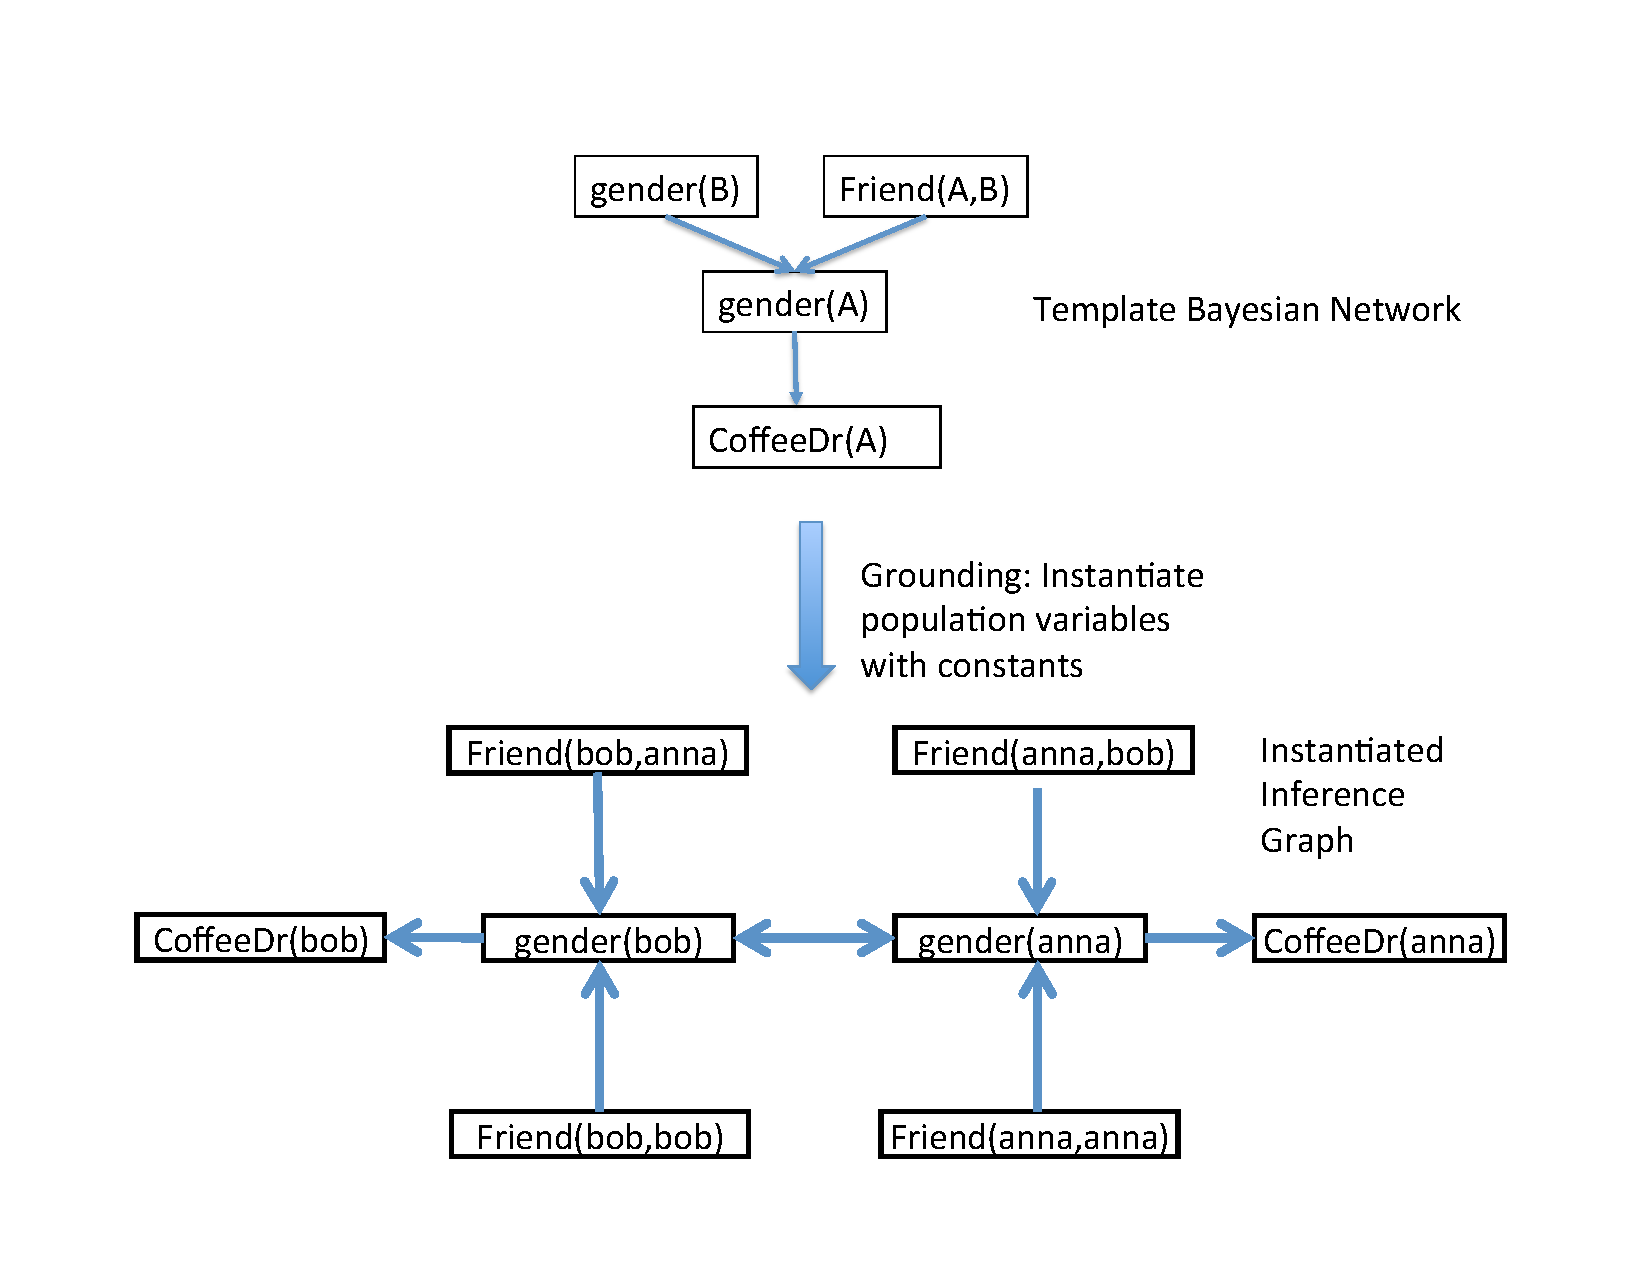
\includegraphics[width = 0.7 \textwidth]{figures/bn}
%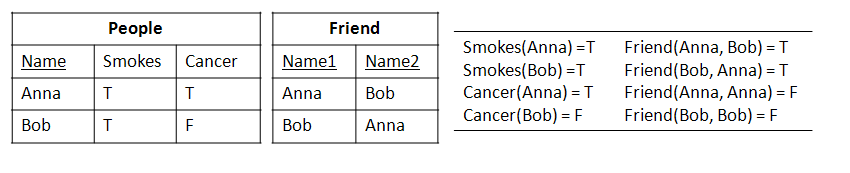
\includegraphics[width=1\textwidth]{database.png}
%}
\caption{A Bayesian network template model (top) and the instantiated inference graph (bottom), with two individuals Anna and Bob in the domain of the first-order or population variables $\A,\B$. Population variables are to be instantiated with all constants that denote a member of the applicable set. The two instantiations $\A\gndlink anna,\B \gndlink bob$ and $\A\gndlink bob,\B\gndlink anna$ produce a cycle involving the two  edges $\it{gender}(anna) \rightarrow \it{gender}(bob)$ and $\it{gender}(bob) \rightarrow \it{gender}(anna)$. \label{fig:bn} \textbf{Add BN parameters as well?}}
\end{center}
\end{figure}


\begin{figure}[htbp]
\begin{center}
%\resizebox{0.78\textwidth}{!}{
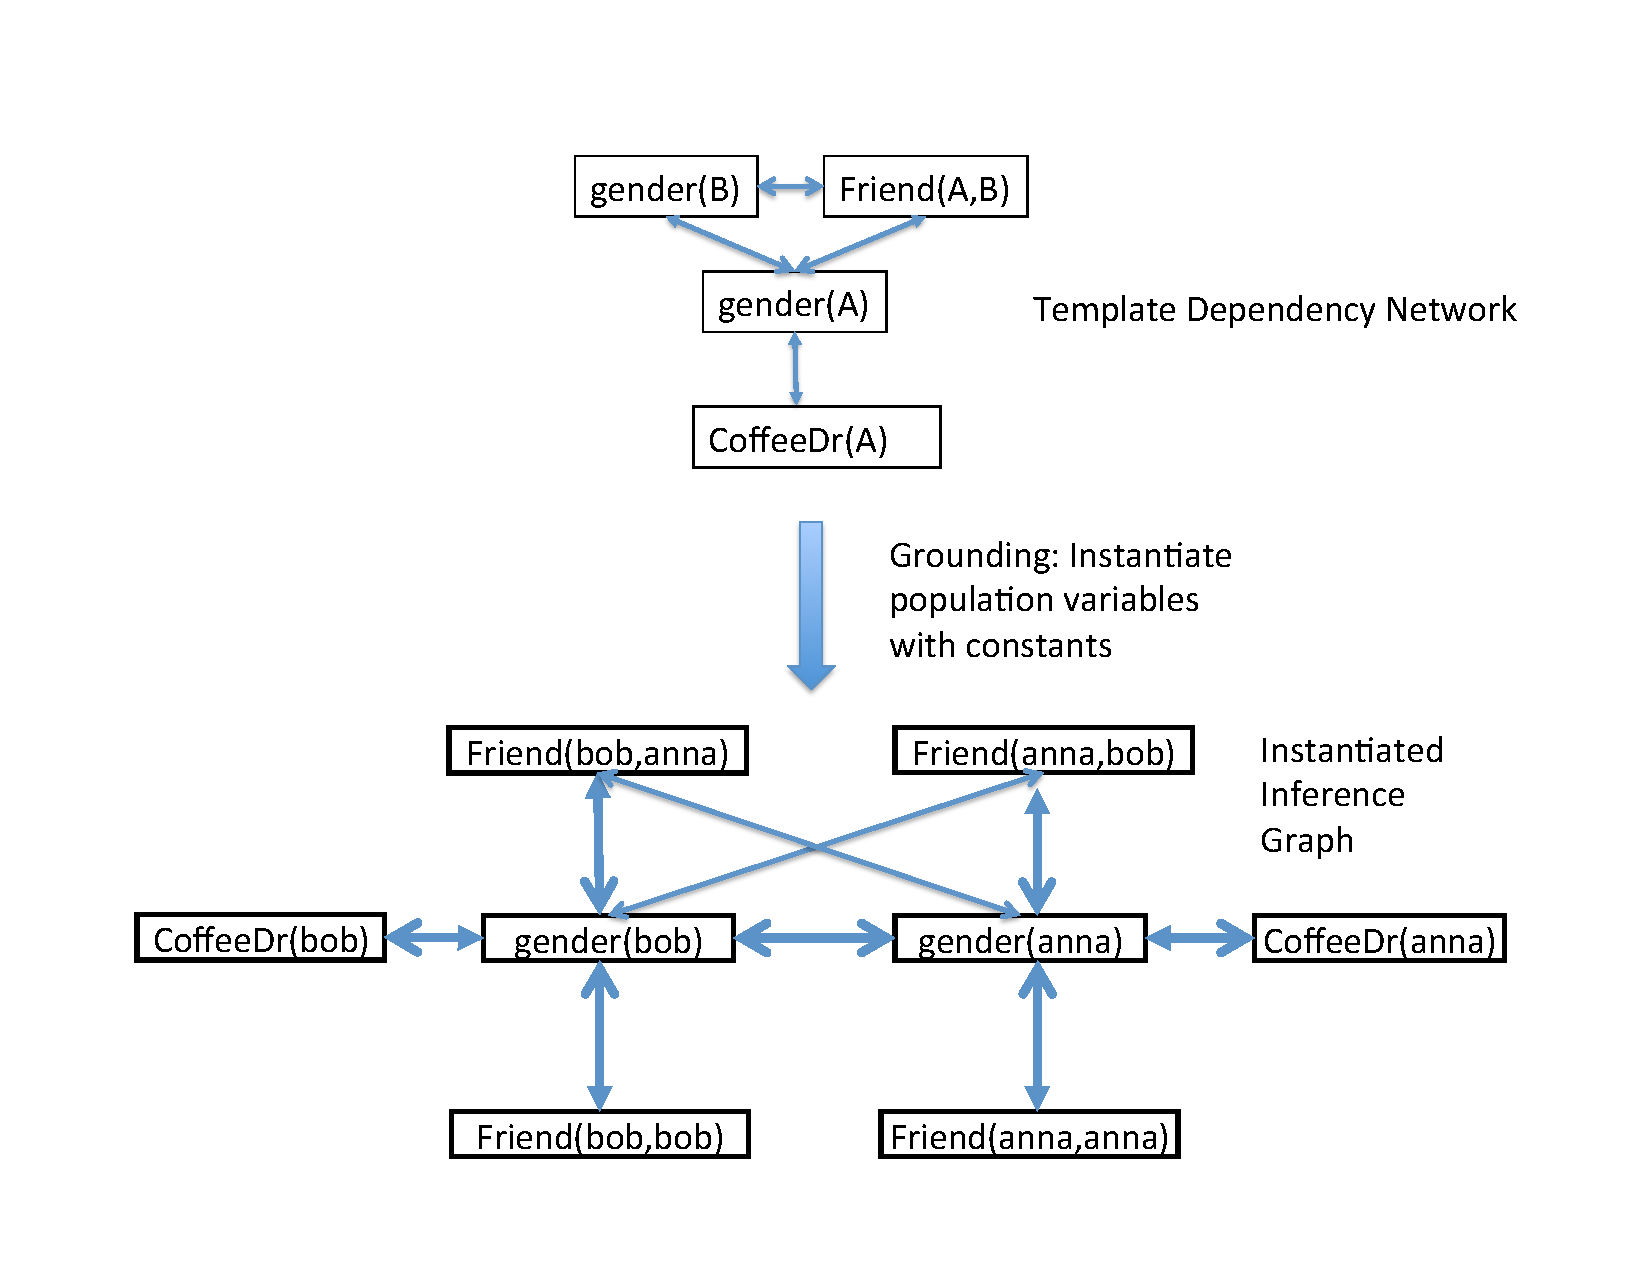
\includegraphics[width = 0.7 \textwidth]{figures/dn}
%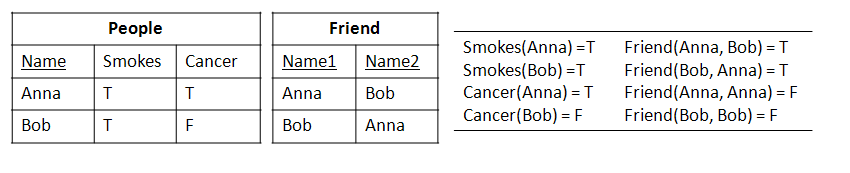
\includegraphics[width=1\textwidth]{database.png}
%}
\caption{A dependency network template model (top) and the instantiated inference graph (bottom). The Gibbs probability parameters for the inference graph specify the conditional probability of a node given its neighbors (Markov blanket). \label{fig:dn}}
\end{center}
\end{figure}

 
\subsection{Relational Dependency Networks} Relational Dependency Networks have received a significant amount of recent development from researchers \cite{Neville2007,Natarajan2012}. Like our paper, this work follows the traditional knowledge-based model construction approach (KBMC). In the KBMC approach, a template graphical model is instantiated for a specific domain of individuals to produce an {\em  instantiated} or {\em ground} graphical model, called the inference graph by Neville and Jensen \cite{Neville2007}. Figures~\ref{fig:bn} and~\ref{fig:dn} illustrate Bayesian/dependency network templates and their groundings.

The advantage of dependency network structure for relational data is that they allow cyclic dependencies. Necessary and sufficient conditions for when a ground Bayesian network template contains cycles are given in \cite{Schulte2012a}.  Typically these occur in the common case that a dataset features auto-correlations, where the value of an attribute for an individual depends on the values of the same attribute for related individuals \cite{Neville2007}. Figure~\ref{fig:bn}  provides an example. In contrast, dependency networks allow cycles, so the grounding of a dependency network template is guaranteed to lead to a valid dependency network structure. The class of cyclic graphs is closed under the operation of grounding, whereas the class of acyclic graphs is not. This fact has been a knotty problem for defining a joint distribution using a template semantics for Bayesian networks ~\cite{Domingos2007,Taskar2002,Getoor2007c}. 

The advantage of the dependency network parametrization for relational data is that conditional probabilities are defined with respect to a larger set of specified nodes. One of the key differences for prediction between relational and non-relational iid data is that {\em different predictors may be instantiated multiple times} \cite{Natarajan2008}. In the social network example of Figure~\ref{fig:bn}, suppose we want to predict the value of the ground node $\it{gender}(anna)$. Each gender of a friend of $\it{anna}$ adds one relevant predictor. The number of predictors is therefore not fixed a priori by the model, but depends on the size of the relational neighborhood, that is, the number of individuals related to the target individual. Relational prediction therefore requires aggregating information from different linked individuals. Two common approaches are using (i) combining rules \cite{Kersting2007} and (ii) aggregation functions \cite{Getoor2007c}. In a dependency network model, the aggregation encompasses the entire Markov blanket of a target node. In a Bayesian network model, the aggregation encompasses only its parents, not the relevant information from its children. We discuss this point further below in Section~\ref{imbalance}. 

 \section{Learning Dependency Networks for Relational Data via Bayesian Networks} Our aim in this paper is combine the fast learning of Bayesian networks with the inference advantages of dependency networks. We utilize state-of-the-art relational learning methods for Bayesian networks. Our novel contribution is a closed-form transformation of a Bayesian network to a relational dependency network. Converting a Bayesian network structure to a dependency network structure is simple: for each node, we add an edge pointing to the node from each member of its Bayes net Markov blanket \cite{Heckerman2000}. The BN Markov blanket of a node consists of its parents, children, and co-parents. The DN structure of Figure~\ref{fig:dn} results from the BN structure of Figure~\ref{fig:bn} in this manner. This is equivalent to the standard moralization  method for converting a BN to an undirected model \cite[12.5.3]{Domingos2007}, \cite{Lauritzen1996}, except that the dependency network contains bi-directed edges instead of undirected edges. 
 
For propositional iid data, converting Bayesian network parameters to dependency network parameters requires solving for the Gibbs conditional probabilities given Bayesian network parameters, which is a standard exercise \cite[Ch.14.5.2]{Russell2010}. The result is the {\em BN log-linear equation} for each node. A discriminative log-linear equation models a conditional probability for a target node value, given an assignment of values to other variables, called the input variables. In the case of a Gibbs probability, the input variables comprise all variables other than the target node. A log-linear model requires defining a set of features, and for each feature a feature function that returns a number for that feature and for a given conditional probability to be computed \cite{Sutton2007}. The parameters of the model are feature weights, one for each feature. The conditional probability of the target node value given values for the input variables is proportional to the exponentiated weighted sum of the feature functions. For propositional data, the  set of features in the BN equation is the set of joint value assignments to a child and its parents in the BN structure. The weights are the log-conditional probabilities of the child value given its parent values. For propositional data, the input variables specify a unique set of values for a given child-parent configuration. But with relational data, multiple value assignments for a child-parent configuration can be instantiated multiple times. Our proposal in this paper is to accommodate multiple instantiations by using the {\em proportion of instantiations} that satisfy a child-parent value assignment as the feature function for the child-parent. Proportions have the desirable consequence that all feature functions are normalized to the [0,1] range. Without this normalization, features with more instantiations carry exponentially more weight.  Figure~\ref{fig:bn-flow} shows the program flow for computing a Gibbs probability using the log-linear equation.

\begin{figure}[htbp]

\begin{center}
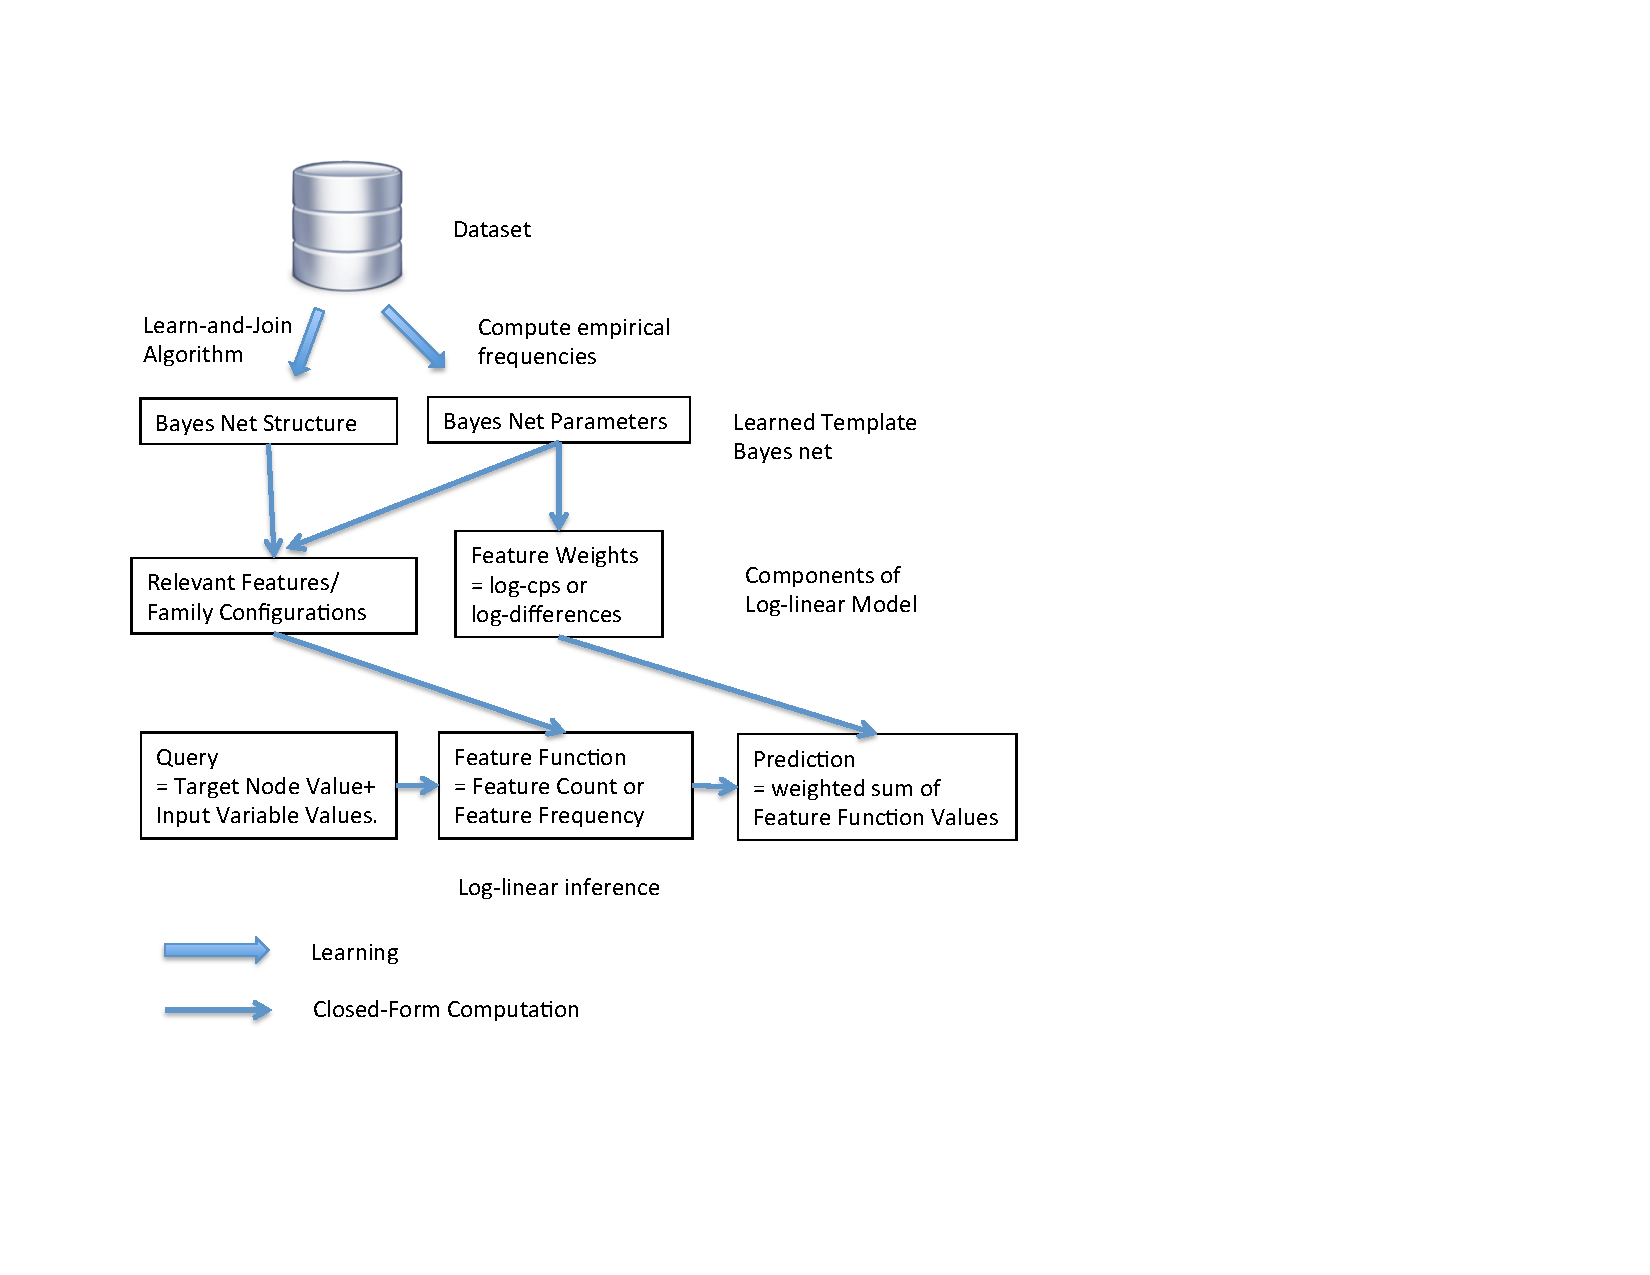
\includegraphics[width=0.7\textwidth]{bn-regress}
\caption{The program flow for computing relational Gibbs probabilities with a template Bayes net. Features and weights are computed from the Bayes net. Feature function values are computed for each query.}
\label{fig:bn-flow}
\end{center}

\end{figure}


[Example needs fixing. Do we want one?: To illustrate, suppose we wish to compute the probability that individual $\A = \it{sam}$ is male, using the template BN of Figure~\ref{fig:bn}~(b).  The input variables specify whether Sam is a coffee drinker, which other persons are his friends, and the gender of other people. There are two parents of the gender node in this template model. One feature in the log-linear model assigns these parents the values $\it{Friend}(\A,\B) = \true$ and $\it{gender}(\B) = \Man$. The feature function returns the proportion of Sam's friends that are male, given the values specified in the input variables. The weight associated with this feature is the log-ratio of two quantities: (i) the conditional probability that $\it{gender}(\A) = \Man$, given the assignment of values to its parents, which is specified as .63 in the BN. (ii) The BN marginal or unconditional probability that $\it{gender}(\A) = \Man$, which can be computed via BN inference as .55. So the weight of this feature is $w = ln(0.63/0.55) \approx 0.136$. The positive weight indicates that according to the BN template model, having a male friend raises the probability of being male. ]

  
\subsection{Evaluation} Using five standard databases, we evaluate the predictive accuracy of dependency networks obtained from Bayesian networks. The parameters of the Bayesian networks are set to be the maximum likelihood estimates. We show that Bayes net learning is fast and scales to databases with millions of records and complex schemas that contain multiple relationships and attributes. We compare predictive accuracy using counts vs. proportions as feature functions.  Proportions yield substantially more accurate predictions, which indicates the importance of normalizing feature functions to a common range. The tested predictions involve different types of target predicates, describing features of individuals,  the existence or absence of links/relationships between individuals, and features of links. To benchmark our approach, we compare BN-to-RDN learning with RDNBoost, the state-of-the art learning method for relational dependency networks. [Results summary] 



\subsection{Contributions} 
Our main contributions are as follows; Figure~\ref{fig:novelty} provides a visual summary.  
\begin{enumerate}
\item A new approach for learning relational dependency networks: learn first a Bayesian network, then convert it to a dependency network.
\item A new log-linear discriminative model for computing the relational dependency network parameters from Bayesian network structure and parameters.
\end{enumerate}

Previous approaches to learning dependency networks take a completely different approach, based on learning a discriminative model for each node that defines Gibbs probabilities directly. The new ideas in this paper can be combined with such approaches in various ways. (1) Functional gradient boosting is also based on a log-linear model. Current approaches use instantiation counts as feature functions. Our results suggest that using using gradient boosting with proportions would achieve better results. (2) Fast Bayesian network learning methods can be used to select features. Discriminative learning methods should work much faster restricted to the BN Markov blanket of a target node. (3) The Bayesian network can provide an initial dependency network for the boosting procedure; gradient boosting can then be used for fine-tuning.

\begin{figure}[htbp]
\begin{center}
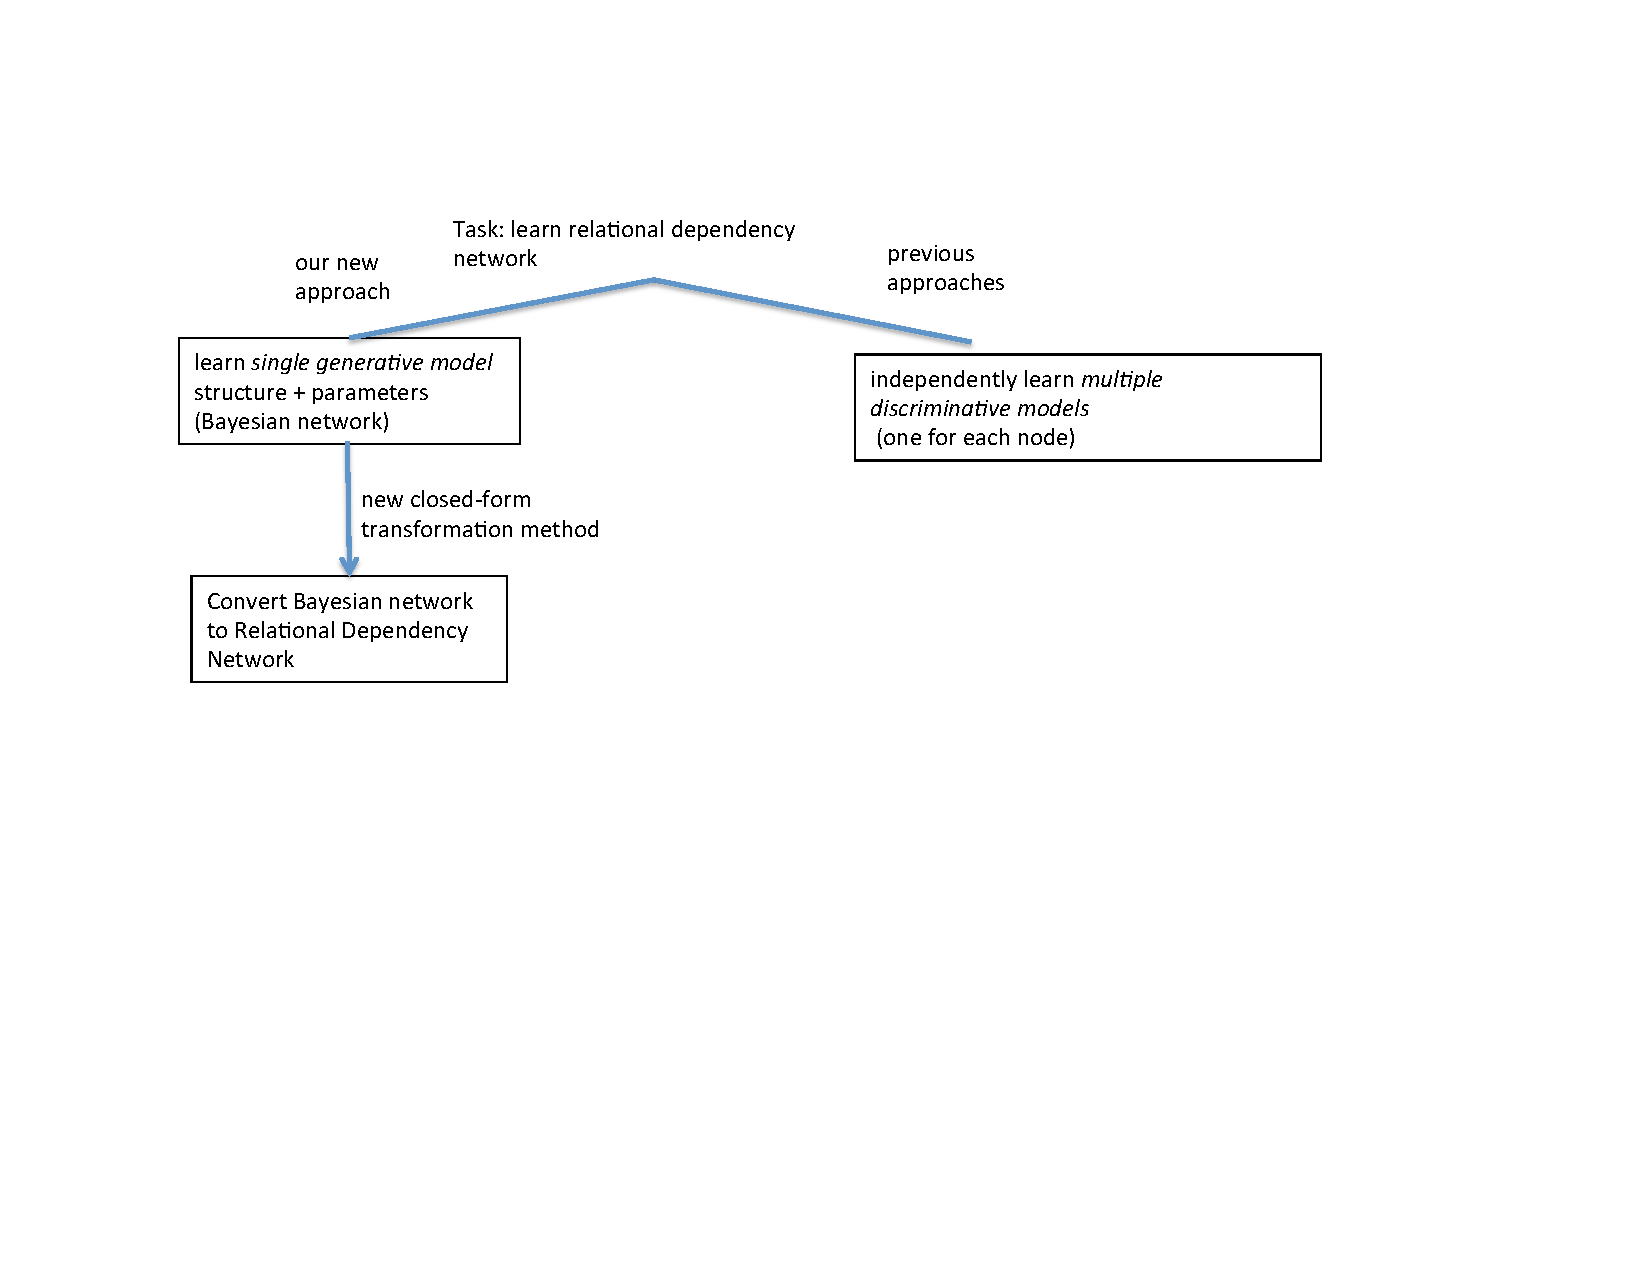
\includegraphics[width=0.7\textwidth]{novelty}
\caption{High-level comparison of our new approach with previous work on learning relational dependency networks.}
\label{fig:novelty}
\end{center}
\end{figure}


\strongpoint{Paper Organization}
We begin (Section~\ref{sec:background}) with background and define the notation for relational Bayes net models.
%, in terms of random selection and ground graphical models. 
% and shows that conditional probabilities maximize the unnormalized likelihood. We then present the frequency regression model. 
Section~\ref{sec:theequation} presents the new log-linear relational regression model, which we evaluate
on five benchmark databases in Sections~\ref{sec:empirical-comparison} and~\ref{sec:general-weights}.
In Section~\ref{sec:rdn-boost} we use the same databases to compare our approach to RDN-Boost \cite{Khot2011}.
We end with related work in Section~\ref{sec:related}, and conclude with suggestions for future work in Section~\ref{sec:conclusion}.

\section{Related Work} \label{sec:related} [Ted: I moved this up for easier review. We can move it back to the end.]

\paragraph{Dependency Network Learning} Dependency networks were introduced by \cite{Heckerman2000}. The traditional approach to learning dependency networks is to learn a collection of discriminative models, one for each node in the network. One motivation for dependency networks is that for nonrelational data, learning multiple discriminative model is faster than learning a single generative model (e.g., a BN). The motivation for our approach is that for large relational data, the reverse is true. The fundamental reason for this is that in relational data, model evaluation is much more computationally expensive relative to  model generation. Parameter estimation and model evaluation in Bayes nets can be done in closed-form using maximum likelihood, rather than through a local optimization procedure as with many discriminative models. Such local optimization procedures require many data accesses to evaluate the model at each optimization step.
Relational model evaluation requires extensive counting computations for finding how often a predictive pattern is instantiated in a given relational neighborhood. In propositional data represented in a single table of cases, instantiation counts cover a subset of already existing table rows. In relational data that are represented in multiple tables, it is necessary to combine information from different tables which involves expensive cross-product. For further  discussion of scalability and model evaluation cost, please see \cite{Neville2007}.

Relational dependency networks were introduced in \cite{Neville2007}. Their learning algorithm used aggregate functions to combine different instantiations of a target node's Markov blanket. Function gradient boosting is the state-of-the-art learning methods for relational dependency networks \cite{Khot2011}. That work uses a log-linear model with counts as feature functions, not proportions. 

We briefly discuss work on Bayesian networks and Markov networks for relational data. \cite{Heckerman2000} {\em et al.} compare Bayes, Markov and dependency nets in detail for nonrelational data. 

\paragraph{Bayesian networks} There are several proposals for defining directed relational template models, based on graphs with directed edges or rules in clausal format \cite{Kersting2007,Getoor2007c,Fierens2009,Milch2007}. In order to define the probability of a child node conditional on multiple instantiations of a parent set, template semantics for Bayesian networks requires the addition of combining rules \cite{Kersting2007} or aggregation functions (usually with extra parameters) \cite{Getoor2007c}. As described by \cite{Kersting2007}, aggregate functions can be added to a Parametrized Bayesian network by including functor nodes with aggregates. Combining rules such as the arithmetic mean~\cite{Natarajan2010} combine global parameters with a local scaling factor, as does our log-linear model. In terms of combining rules,  our model uses the {\em geometric mean} rather than the arithmetic mean.\footnote{The geometric mean of a list of numbers $x_{1},\ldots,x_{n}$ is $(\prod_{i} x_{i})^{1/n}$. The logarithm of the geometric mean is therefore $1/n \sum_{i} \ln x_{i}$. Thus geometric mean = exp(average (logs)).} To our knowledge, the geometric mean has not been used before as a combining rule for relational data.  Another difference with template Bayesian networks is that the geometric mean is applied to the entire Markov blanket of the target node, whereas usually a combining rule applies only to the parents of the target node. 

\paragraph{Markov Networks} Markov Logic Networks (MLNs) provide a logical template language for undirected graphical models. 
Richardson and Domingos propose transforming a Bayesian network to a Markov Logic network using moralization, with log-conditional probabilities as weights \cite{Domingos2007}. 
This is also the standard Bayes net-to-MLN transformation recommended by the Alchemy system \cite{bib:bayes-convert}. A discriminative model can be derived from any MLN.  The Gibbs conditional probabilities defined by an MLN obtained from converting a Bayesian network are the same as those defined by our log-linear equation, when {\em counts} are used as feature function \cite{Schulte2011}. There is no MLN whose discriminative model is equivalent to our log-linear equation with {\em proportions} as feature functions.  
 
\section{Background: Bayes Nets for Relational Data} \label{sec:background} [Question: can we get away with having only the notation table + examples?] [Suggestion: we should probably use constrained instantiation count because of the similarity to Poole's parfactors.]

We adopt function-based notation from logic for combining Bayes nets with relational concepts \cite{Russell2010,Poole2003,Getoor2006,Chiang2012}. Different communities in statistics and logic use different terms for similar concepts, and similar terms for different concepts. We strive for notation that is as broadly accessible as possible. Table~\ref{table:relational-notation} summarizes our notation for relational concepts. %, and note conflicts of terminology when we cannot avoid them. 


\begin{table}[htbp]

\caption{Summary of Notation for Relational Concepts}
\begin{tabular}{lp{8cm}p{5cm}}\label{table:relational-notation}
Notation & Explanation & Example \\\hline
$\A,\B$ & \defterm{Population Variables} & $\A$\\
$\TT, \UT, \VT$ & \defterm{Terms}. A term consists of a \defterm{functor} and its arguments.  The arguments may be any combination of 
\defterm{population variables} and \defterm{constants}. & $\it{gender}(\A)$ \\
$\TF, \UF, \VF $ & \defterm{Term Tuples}.  A list of terms. A given term can occur at most once. Order is significant. & $\it{gender}(\B); \it{Friend}(\A,\B)$\\ $\Range{\TT}, \Range{\TF}$ & The \defterm{range of a term} and the \defterm{range of a term tuple}. The range of a \defterm{term} is the range of its functor. The range of a tuple is the Cartesian product of the ranges of the constituent \defterm{terms}.& $\Range{\it{gender}(\B), \it{Friend}(\A,\B)} = \{\Woman,\Man\} \times \{\true,\false\}$ \\
$\TV, \UV, \VV$ & \defterm{Values} from the ranges of $\TT, \UT, \VT$. & $\Man;\true$ \\
$\TTuple, \UTuple, \VTuple$ & \defterm{Tuples of values} from the ranges of $\TF, \UF, \VF$. & $(\Man,\true)$ \\
%$\Vars{\TT}, \Vars{\TF}$ & The \defterm{variables of a term} and the \defterm{variables of a vector}. A list of all the %unique 
%population variables in a term or vector. & $\Vars{\it{Friend}(\A,\B)} = \{\A,\B\}.$ \\
$\TT = \TV$ & \defterm{Literal}. A term bound to a value from its range. 
& $\it{Friend}(\A,\B) = \true$ \\
$\TF = \TTuple$ & \defterm{Literal conjunction}. A conjunction bound to a tuple of values from its \defterm{range}. Every \defterm{term} in a literal conjunction is bound to its corresponding value. & $\it{Friend}(\A,\B) = \true$,$\it{gender}(\A)=\Woman$\\
%A single \defterm{grounding} may be applied to all terms in the conjunction. \\
$\grounding$ %, $\{\A_{i}\gndlink\a_{1},\ldots,\A_{j}\gndlink \a_{j}\}$ 
& \defterm{Instantiation}.
%$\grounding: \TF \rightarrow \PG{\TF}$ & \defterm{Grounding}. 
An instantiation maps zero or more \defterm{population variables} to appropriate \defterm{constants}.  & $\grounding = \{\A\gndlink anna,\B\gndlink bob\}$
%We will typically assume groundings, implying them in the $\PG{\TF}$ and $\FG{\TF}$ notations. 
 \\
$\FG{\TT}, \FG{\TF}$ & \defterm{Fully ground term/tuple}. All arguments to all functors are constants. Equivalently, the term/tuple does not contain any population variables. & $\it{gender}(anna),\it{Friend}(anna,bob)$ \\
$\DB$ & %\defterm{Database}. A 
Complete \defterm{literal conjunction} comprising \defterm{fully grounded} terms.
The conjunction binds {\em every} ground term to a value. & See Table~\ref{table:count-examples}.
%$\it{gender}(anna) = W$, $\it{gender}(bob) = M,$ $\it{Friend}(anna,bob) = \true,$ $\it{Friend}(bob,anna) = \true,$ $\it{Friend}(anna,anna) = \false,$ $\it{Friend}(bob,bob) = \false$
%For \defterm{literal terms} whose \defterm{ranges} are boolean, we assume that any fully ground instance absent from the database has the value $\false$. For a given computation of \defterm{Gibbs conditional probability}, the database is fixed and does not contain the term for which the probability is being computed. 
\\
$\Count{\TF = \TTuple}{\DB}$ & \defterm{Instantiation Count.}  Counts the number of groundings of $\TF = \TTuple$ that evaluate as true in $\DB$. A \defterm{grounding} instantiates {\em all} population variables in $\TF$.  & 
%$\Count{\it{gender}(\A) = \Woman, \it{Friend}(\A,\B) = \true}{\DB}$ = 1. 
See Table~\ref{table:count-examples}.\\
\end{tabular}
\end{table}


\subsection{Relational Concepts.} A  \defterm{population} $\population$ is a set of individuals. Individuals are denoted by lower case identifiers (e.g., $\it{sam}$). Identifiers representing individuals are called \defterm{constants}. 

\subsubsection{Functor Notation}
A \defterm{functor}
$
\functor: \population_{1},\ldots,\population_{a} \rightarrow \outdomain_{\functor}
$
maps a list of individuals to a functor value, 
where $\outdomain_{\functor}$ is the output type or \defterm{range} of the functor. In this paper we consider only functors with a finite range.
%, disjoint from all populations.  
If $\outdomain_{\functor} = \{\true,\false\}$, the functor $\functor$ is a (Boolean) \defterm{predicate}; other functors are called \defterm{attributes}. A predicate with more than one argument is called a \defterm{relationship}. Predicates typically represent the presence of a binary property or a relationship, while attributes typically represent properties that can take multiple values. 
%The finite-ranged attributes considered in this paper are syntactic sugar: they could be systematically replaced by sets of unary predicates, such as replacing $\it{gender}$ with $\it{Man}$ and $\it{Woman}$. 
% OS: this would change the learning behaviour, see Domingos and our AAAI paper.
We use lowercase for attribute functors and uppercase for predicates.
We define two kinds of variables, with distinct domains: (i) A \defterm{population variable} varies over a population domain. The same population may be associated with more than one population variable. We use an outline Latin font for population variable ($\A,\B,\ldots$).
%We index population variables if more than one is associated with the same population (e.g., $\A, \B, \it{Student}$). 
(ii) A \defterm{term}
is an expression of the form $\functor(\terms) \equiv \functor(\term_{1},\ldots,\term_{k})$, where 
each $\term_{i}$ is a population variable or a constant of the appropriate argument type for that functor.\footnote{The traditional term in first-order logic for a term variable is ``function term''. In statistical-relational learning, alternative terms include ``parametrized random variable'' \cite{Poole2003}, ``atom'' \cite{Chiang2012}, ``Bayesian atom''  \cite{Kersting2007}, and ``functor random variable'' \cite{Schulte2012}.} A term can be assigned values in the range of its functor.

In a context where the functor and arguments of terms are not important, we denote them by uppercase Latin letters ($\TT,\UT,\ldots$).

A \defterm{literal} is an assignment to a term, denoted generically as $\TT = \TV$, where $\TV$ is in the range of the functor for $\TT$. 
% where $v$ is in the range of $\functor$ and $\functor(\term_{1},\ldots,\term_{a})$ is a PRV. 
Literals can be combined to generate \defterm{formulas}. 
In this paper we consider only formulas that are \defterm{conjunctions} of literals, denoted by the Prolog-style comma notation, e.g., 
%$\functor(\term_{1},\ldots,\term_{a}) = v, \ldots,\functor_{z}(\term'_{1},\ldots,\term'_{a'}) = v'$. The corresponding more compact notation for a conjunctive formula would be 
$\TT = \TV, \ldots, \UT = \UV$, for which we also use the  vector notation $\TF = \TTuple$.


\subsubsection{Groundings and Relational Structures}
An term is \defterm{ground} if it contains no population variables. We mark fully ground terms and formulas by an asterisk, $\FG{\TT}$. An \defterm{instantiation}  for a term assigns a constant to a set of the population variables in the term. Formally, an instantiation $\gamma$ is a set $\{\A_{i}\gndlink\a_{1},\ldots,\A_{j}\gndlink \a_{j}\}$ 
that assigns a constant $\gamma(\A_{i})$ to each variable $\A_{i}$ from its population. The expression $\Ground{\TT}$ denotes the term that results from applying the substituition $\gamma$ to all variables in $\TT$. If the instantiation $\gamma$ specifies a constant for all the population variables that occur in the term, the resulting term is ground, and $\gamma$ is called a \defterm{grounding}. An instantiation is applied to a formula by applying it to all terms in the formula. Thus a grounding of a formula is an instantiation that grounds of all its terms.


A \defterm{relational structure} is a (model, interpretation) pair that assigns a unique value to each ground term \cite{Chiang2012}. Assuming a finite list of functors, and that all populations are finite, a relational structure is equivalent to a \defterm{complete conjunction} of ground literals $\DB \equiv (\FG{\TF} = \TTuple)$. The ground literals in the relational structure are called \defterm{facts}. A conjunction of ground literals evaluates as true in a relational structure if each of its conjuncts is a fact. A well-studied operation~\cite{Schulte2013} for statistical learning is to count, for a given nonground formula $\TF = \TTuple$ and complete conjunction $\DB$, the number of groundings of the formula that evaluate as true in the complete conjunction. Note that only groundings that instantiate exactly the population variables that appear in $\TF$. We refer to this quantity as the formula's \defterm{instantiation count}, denoted by $$\Count{\TF = \TTuple}{\DB}.$$

\subsubsection{Examples.}

Figure~\ref{fig:pbn}(a) shows the facts in a relational structure, represented as database tables. For this example only, let us assume that the tables represent a relational structure completely, and hence specifies a complete conjunction $\DB$. Table~\ref{table:count-examples} shows examples of instantiation counts for this complete conjunction.

\begin{table}[htdp]
\caption{Instantiation counts in the database of Figure~\ref{fig:pbn}. For the sake of the example, we treat the database as specifying a complete conjunction $\DB =$  $\{gender(anna) = W$,  $gender(bob) = M$, $Friend(anna,bob) = T$, $Friend(bob,anna) = T$, $Friend(anna,anna) = F$, $Friend(bob,bob) = F
\}$.}
\begin{center}
\begin{tabular}{lc}
Formula & Instantiation Count\\\hline
$\it{gender}(\A) = \Man$ & 1 \\
$\it{Friend}(\A,\B) = \true$ & 2\\
$\it{Friend}(bob,\B) = \true$ & 1 \\
$\it{gender}(\B) = \Man, \it{Friend}(\A,\B) = \true$ & 1 \\
$\it{gender}(anna) = \Man, \it{Friend}(\A, anna) = \true$ & 0
\end{tabular}
\end{center}
\label{table:count-examples}
\end{table}%


\begin{table}

\caption{Summary of Notation for Template Bayes Nets}
\begin{tabular}{lp{8cm}p{4cm}}\label{table:BN-notation}
Notation & Explanation & Example  \\\hline
$\Pa{\TT}: \TT \rightarrow \TF$ & \defterm{Parents}. The \defterm{terms} associated with the parent nodes of the unique Bayes net node associated with $\TT$. The parent terms will be distinct. & $\Pa{\it{gender}(\A)}$ = $\langle\it{gender}(\B),\it{Friend}(\A,\B)\rangle$
%Any \defterm{grounding} applied to $\TT$ will also be applied to $\TF$. 
\\
$\Ch{\TT}: \TT \rightarrow \TF$ & \defterm{Children}. The \defterm{terms} associated with the child nodes of the unique Bayes net node associated with $\TT$. 
& $\Ch{\it{gender}(\A)}$ = $\it{CoffeeDr}(\A)$
%Any \defterm{grounding} applied to $\TT$ will also be applied to $\TF$.
\\
%$\Mrange{\TT}$ & \defterm{Value in the Markov range}. Tuple of values from $\Range{\MB{\TT}}$. \\
$\Prange{\TT}$ & \defterm{Value in the parent range}. Tuple of values from $\Range{\Pa{\TT}}$. & $\langle \Man,\true \rangle$\\
%$\jprob{\TF = \TTuple[0.6ex]}$ & \defterm{Joint probability} of a literal conjunction. \\
$\TT=\TV,\Pa{\TT} = \Prange{\TT}$ & \defterm{Family Configuration} that specifies values for node $\TT$ and its parent nodes $\Pa{\TT}$. & $\it{gender}(\A) = \Man,$ $\it{gender}(\B) = \Woman,$ $\it{Friend}(\A,\B) = \true$\\
$\cprob{\TT = \TV}{\Pa{\TT} = \Prange{\TT}}$ & \defterm{Conditional probability} of a node value given a parent configuration. & $\cprob{\it{gender}(\A) = \Woman}{\it{gender}(\B) = \Woman,\it{Friend}(\A,\B) = \true}$ = $0.55$
\\
%$\cprob{\TT = \TV}{\UF = \UTuple}$ & \defterm{Conditional probability} of a literal term given a literal conjunction.  \\
$\jprob{\TT = \TV}$ & \defterm{Marginal probability} of a node value entailed by the Bayes net. & $P(\it{gender}(\A)= \Man)$ = $0.55$
\end{tabular}
\end{table}


\subsection{Bayes Nets for Relational Data.} \label{sec:graph-relational}




A Bayes net (BN) is a pair
$\langle{G,\bs{\theta}_G}\rangle$, where $G$ is a directed acyclic graph and $\bs{\theta}_G$ is a set of parameters that specify the  probability distributions of children conditional on instantiations of their parents. A \defterm{Template Bayes Net} (TBN) is a Bayes net whose nodes are nonground terms~\cite{Poole2003,Schulte2011}. That is, every node in the Bayes net is a term containing one or more population variables. When describing Bayes nets, we use ``term'' and ``node'' interchangeably. Table~\ref{table:BN-notation} summarizes our notation for Bayes nets and Figure~\ref{fig:pbn}(b) shows an example net.

A \defterm{family} comprises a node and its parents. A \defterm{family configuration} specifies a value for a child node and each of its parents. Since we consider functors with discrete ranges only, there are only finitely many family configurations. Using the notation in Table~\ref{table:BN-notation}, a family configuration is equivalent to the conjunction $\TT=\TV,\Pa{\TT} = \Prange{\TT}$. For each family configuration, a \defterm{Bayes net parameter} $$\cprob{\TT = \TV}{\Pa{\TT} = \Prange{\TT}}$$ specifies the probability of the child value $\TV$ given the parent values $\Prange{\TT}$.\footnote{For \iid{} data, a commonly  used notation for a BN parameter is $\theta_{ijk}$~\cite{Heckerman1998}.} Given a complete conjunction $\DB$, the number of family configurations is\footnote{For \iid{} data, a commonly  used notation for this quantity is $\instances_{ijk}$~\cite{Heckerman1998}.} $$\Count{\TT=\TV,\Pa{\TT} = \Prange{\TT}}{\DB}.$$



\subsection{Bayes Net Gibbs Probabilities.}

We review the equation for Gibbs conditional probabilities for a Bayes net that specifies a joint distribution over its nodes via the standard product formula \cite{Pearl1988}. 
Inferring a Gibbs conditional probability can be represented as a probabilistic query
$$\Gprob{\TT = \TV} {\VF = \VTuple} = ?$$
\noindent where $\TT$ is the target node, $\TV$ is a value for the target node, and $\VTuple = \VF$ specifies a value for every other node. The product formula for the Bayes net joint distribution entails that the Gibbs probability is proportional to a product of conditional probabilities for the target node and its children~\cite[Ch.14.5.2]{Russell2010}:  
\begin{equation} \label{eq:bn-mb-product}
\Gprob{\TT = \TV} {\VF = \VTuple} \propto \prod_{\UT \in \{\TT\} \cup \Ch{\TT}} \cprob{\UT = \UV}{\Pa{\UT} = \Prange{\UT}}
\end{equation}
where $\UV$ and $\Prange{\UT}$ are specified by the values in $\TV,\VTuple$ for the corresponding nodes. The product is a number between 0 and 1 that needs to be normalized to obtain the Gibbs conditional probability.

\strongpoint{Example} For the Bayes net of Figure~\ref{fig:pbn}, consider the query

$$\Gprob{\it{gender}(\A) = \Woman} {\it{gender}(\B) = \Woman, \it{Friend}(\A,\B) = \true, \it{CoffeeDr}(\A) = \true}.$$

\noindent By Equation~\ref{eq:bn-mb-product}, this probability is proportional to 

\begin{eqnarray*}
\cprob{\it{gender}(\A) = \Woman}{\it{gender}(\B) = \Woman, \it{Friend}(\A,\B) = \true} & \cdot & \cprob{\it{CoffeeDr}(\A) = \true}{\it{gender}(\A) = \Woman} \\
= 0.55 &\cdot &0.8 = 0.44.
\end{eqnarray*}


\subsection{Log-Linear Models}

Equation~\ref{eq:bn-mb-product} can be seen as an instance of a standard log-linear schema as follows. The general equation form that defines a \textbf{discriminative log-linear model} \cite[Sec.4.2.2.1]{Sutton2007} is 

\begin{equation} \label{eq:log-linear}
\Gprob{\TT = \TV} {\VF = \VTuple} \propto exp(w_{\TV} + \sum_{i=1}^{K} w_{i} f_{i}(\TV,\VF)),
\end{equation}

\noindent where $\TT$ is the target or output variable, and $\VTuple = \VF$ represents an assignment of values to the input variables. The model is based on a finite set of $K$ features, and for each feature there is a real-valued weight parameter $w_{i}$. The term $w_{\TV}$ is a bias weight that may depend on the target node value $\TV$ but not the input variables. The functions $f_{1},\ldots,f_{k}$ are \textbf{feature functions}, such that $f_{i}$ returns a real number for feature $i$ given values for both the target and input variables. A log-linear equation defines a log-linear model; we use the term ``equation'' to emphasize the mathematical form, and the term ``model'' to emphasize the parameter space.

Rewriting Equation~\ref{eq:bn-mb-product} as 

\begin{equation} \label{eq:bn-mb}
\Gprob{\TT = \TV} {\VF = \VTuple} \propto exp(\sum_{\UT \in \{\TT\} \cup \Ch{\TT}} \ln\cprob{\UT = \UV}{\Pa{\UT} = \Prange{\UT}})
\end{equation}

\noindent shows that a BN Gibbs probability follows a log-linear model with the following specifications. (1) The features are all family configurations whose child node is either the target node or a child of the target node. (2) The feature weights are the log-conditional probabilities associated with a family configuration; the bias weight is 0. (3) The feature function for each a family configuration returns 1 if the family configuration is specified by the conjunction $(\TV,\VTuple)$ of input and output variables, 0 otherwise. 

This log-linear equation specifies the Gibbs probability for the nonground terms/nodes in the template Bayes net. Our goal in this paper is to define inference for queries whose target are ground terms. We therefore want to generalize Equation~\eqref{eq:bn-mb} for ground terms. The log-linear equations for ground terms that we consider are also based on products of the Bayes net parameters, combined with transformations. 



\section{The Log-Difference Frequency Equation} 
\label{sec:theequation}

\begin{table}

\caption{Summary of Notation for Relational Gibbs Probabilities}
\begin{tabular}{lp{4cm}p{4cm}}\label{table:equation-notation}
Notation & Explanation & Example \\\hline
$\FG{\Ground{\TI}}$ & Fully Ground Target Node & $[\it{gender}(\A)]_{\{\A\gndlink sam\}} = \it{gender}(sam) $ \\
$\TV$ & Target Node Value & $\Man$\\
$\QC$ & \defterm{Query Conjunction.} A fully ground literal conjunction that binds every term to a value except for the target node & See Table~\ref{table:count-examples}\\
$\Gprob{\FG{\Ground{\TI}} = \TV} {\QC}$ & \defterm{Gibbs conditional probability}, or a \defterm{Query} & $\Gprob{\it{gender}(sam) = \Man}{\QC}$ \\
$\Appendterm{\Ground{\UI}  = \UV} {\Ground{\Pa{\UI}} = \Prange{\UT}}$ & Partially ground query family configuration &  $\it{gender}(sam) = \Man,$ $\it{gender}(\B) = \Woman,$ $\it{Friend}(sam,\B) = \true$\\
$\Relcount{\Appendterm{\Ground{\UI}  = \UV} {\Ground{\Pa{\UI}} = \Prange{\UT}}} {\QC,\Ground{\TI} = \TV}$ & \defterm{Relevant Instantiation Count} of a query family configuration. & See Section~\ref{sec:predictors}. \\
$\Relfreq{\Appendterm{\Ground{\UI}  = \UV} {\Ground{\Pa{\UI}} = \Prange{\UT}}} {\QC,\Ground{\TI} = \TV}$ & \defterm{Relevant Instantiation Frequency} of a query family configuration. & See Section~\ref{sec:predictors}. \\


%$\RelcountC{\UT=\UV,\Pa{\UT} = \Prange{\UT}}{\QC,\Ground{\TI} = \TV}{\grounding}$ & \defterm{Constrained Count of Relevant Instantiations} of a query family configuration. & See the text. \\
%$\RelfreqC{\UT=\UV,\Pa{\UT} = \Prange{\UT}}{\QC,\Ground{\TI} = \TV}{\grounding}$ & \defterm{Constrained Frequency of Relevant Instantiations} of a query family configuration. & See the text. \\
%$\Relfreq{\TF}{\DB}$ & \defterm{Relevant frequency} of a \defterm{conjunction}, given a \defterm{database}. See the text for the definition of relevant frequency. \\& $\it{gender}(\A)$ \\
\end{tabular}
\end{table}


%In this section we generalize Equation~\ref{eq:bn-mb} to the relational case. 
We propose a log-linear equation for computing a Gibbs conditional probability in closed form, given (i) a ground target node (the output variable), (ii) a target value for the target node, (iii) a complete set of values for all ground terms other than the term of the target node (the input variables), and (iv) a template Bayes net. We refer to our proposal as the 
\defterm{log-difference frequency equation}. Our notation is summarized in Table~\ref{table:equation-notation}. For now we assume that component~(iv), the template BN, is fixed (Section~\ref{sec:predictors} discusses structure learning), and consider in this section components~(i)--(iii). 
%The features and weights can be computed in closed-form from the BN template, and the feature functions from the BN template and the given query. 
Figure~\ref{fig:bn-flow} shows the program flow for computing a Gibbs probability using the log-difference frequency equation.

% We begin with components~(i)--(iii) and introduce component~(iv), the template net, in Section~\ref{sec:predictors}.
% 



 \subsection{Conditional Queries} Conditional queries comprise the following elements:
 
\begin{enumerate}
\item A \defterm{target literal} $\FG{\Ground{\TI}} = \TV$, where $\FG{\Ground{\TI}}$ denotes a ground term that results from applying the grounding $\grounding$ to the term $\T$.
\item A conjunction $\DB$ that specifies a value for each ground term other than $\FG{\Ground{\TI}}$. The conjunction $(\Qconj)$ specifies the value of {\em every} ground term; we refer to it as the \defterm{query conjunction}.
\end{enumerate}

A Gibbs conditional probability corresponds to a probabilistic \defterm{query}

$$\Gprob{\FG{\Ground{\TI}} = \TV} {\DB} = ?$$

\noindent For example, a target node may be $\it{gender}(sam)$, which results from the grounding $\it{gender}(\A)\{\A\gndlink sam\}$.\footnote{The node $\it{gender}(sam)$ can also be defined by the grounding $\it{gender}(\B)\{\B\gndlink sam\}$. To make our definition unambiguous, we assume that the BN is in main functor format and that the template node $\T$ is the main functor node for its functor; see \cite{Schulte2012a}.}  The conjunction $\DB$ specifies a value for all ground terms other than $\it{gender}(sam)$.

\subsection{Features and Feature Weights} \label{sec:features} The features are all family configurations whose child node is either the target node or a child of the target node, as with nontemplate BNs. Thus the set of features equals the set of \defterm{query family configurations}

$$\QFC \equiv \{\Appendterm{\UI  = \UV} {\Pa{\UI} = \Prange{\UT}}: \UT \in \{\TT\} \cup \Ch{\TT}, \UV \in \Range{\UT}, \Prange{\UT} \in  \Range{\Pa{\UT}}\}.$$

 For each query family configuration 
there is an associated weight $$w \equiv  \ln \cprob{\UT = \UV}{\Pa{\UT} = \Prange{\UT}}  .$$ 
%\end{enumerate}
%
If $\cprob{\UT = \UV}{\Pa{\UT} = \Prange{\UT}} = \ln \jprob{\UT = \UV}$, then the parent configuration is probabilistically independent of the child condition (according to the template BN). In that case we say that the feature defined by the family configuration is \defterm{irrelevant}, otherwise \defterm{relevant}. In the log-difference equation, irrelevant features receive weight 0, which is equivalent to eliminating them from the model. Table~\ref{table:relevance} illustrates relevant and irrelevant features.


\point{Discussion} It is well-known that eliminating irrelevant features is important for predictive accuracy in statistical-relational learning \cite{Getoor2007c,Ngo1997,Natarajan2008,Heckerman+al:SRL07}. For example, individuals whose every relationship with the target individual has value $\false$ are often irrelevant to predicting features of the target. In the example above, the gender of nonfriends (all $\B$ such that $\it{Friend}(sam, \B) = \false$) is probabilistically independent of the gender of the target. In a realistic social network, where 99\% or more of the users are {\em not} friends with a given individual, this would entail that the vast majority of groundings are irrelevant to predicting an individual's gender. A common approach to eliminating irrelevant predictors
%to related entities 
is to stipulate a logical condition that must be met for the predictor to be included~\cite{Ngo1997,Natarajan2008,Russell2010,Getoor2006}. The log-difference model instead defines irrelevant features in terms of the Bayes net parameters, and eliminates them by assigning 0 weight.
%, which is easier to incorporate into a log-linear model than a logical condition.


\begin{table}
\caption{Relevant and Irrelevant Features, or Family Configurations, for the Bayes net of Figure~\ref{fig:pbn}. Marginal probabilities are computed using standard Bayes net inference.}
\begin{center}
%\resizebox{1\textwidth}{!}{
 \begin{tabular}{@{} |c p{2cm}|p{3.5cm} p{2cm}|c|@{}}
 \hline
Child Node Value & Marginal Probability & Parent configuration & Conditional Probability & Relevant? \\\hline
$\it{CoffeeDr}(\A) = \true$ & 0.70 & $\it{gender}(\A) = \Woman$ & 0.80 & yes \\
$\it{gender}(\A) = \Woman$ & 0.45 & $\it{gender}(\B) = \Woman,$ $\it{Friend}(\A,\B) = \false$ & 0.45 & no \\\hline
\end{tabular}
%}
\end{center}
\label{table:relevance}
\end{table}%

%Notice that the weight is computed with respect to the conditional probabilities for the {\em unground} template nodes $\UT$ and $\Pa{\UT}$. This implements a form of parameter tying where instantiations of the template inherit its parameters~\cite{getoor-intro}.


\subsection{Feature Functions} \label{sec:predictors}
For each feature, a feature function maps the query conjunction to a real number. A common feature function choice in log-linear models is the number of times that the feature is instantiated in the query conjunction. 
%This feature function corresponds to the \defterm{family configuration count}. 
Our basic proposal is to use, instead, the {\em frequency} with which each feature
%family configuration 
is instantiated in the query conjunction. 
%We refer to this feature function as the \defterm{family configuration frequency}. 
%
To compute feature frequencies, we first compute feature counts, then normalize.
%The family configuration frequency is the number of family configuration counts, divided by the number of possible instantiations for the given ground target node. 
To count all and only instantiations that are related to the grounding of a target node, we apply the grounding to its parents, children, and co-parents, as illustrated in Figure~\ref{fig:regress}. 


%\point{(1) Apply the query grounding} 
\begin{figure}

\begin{center}
\resizebox{0.4\textwidth}{!}{
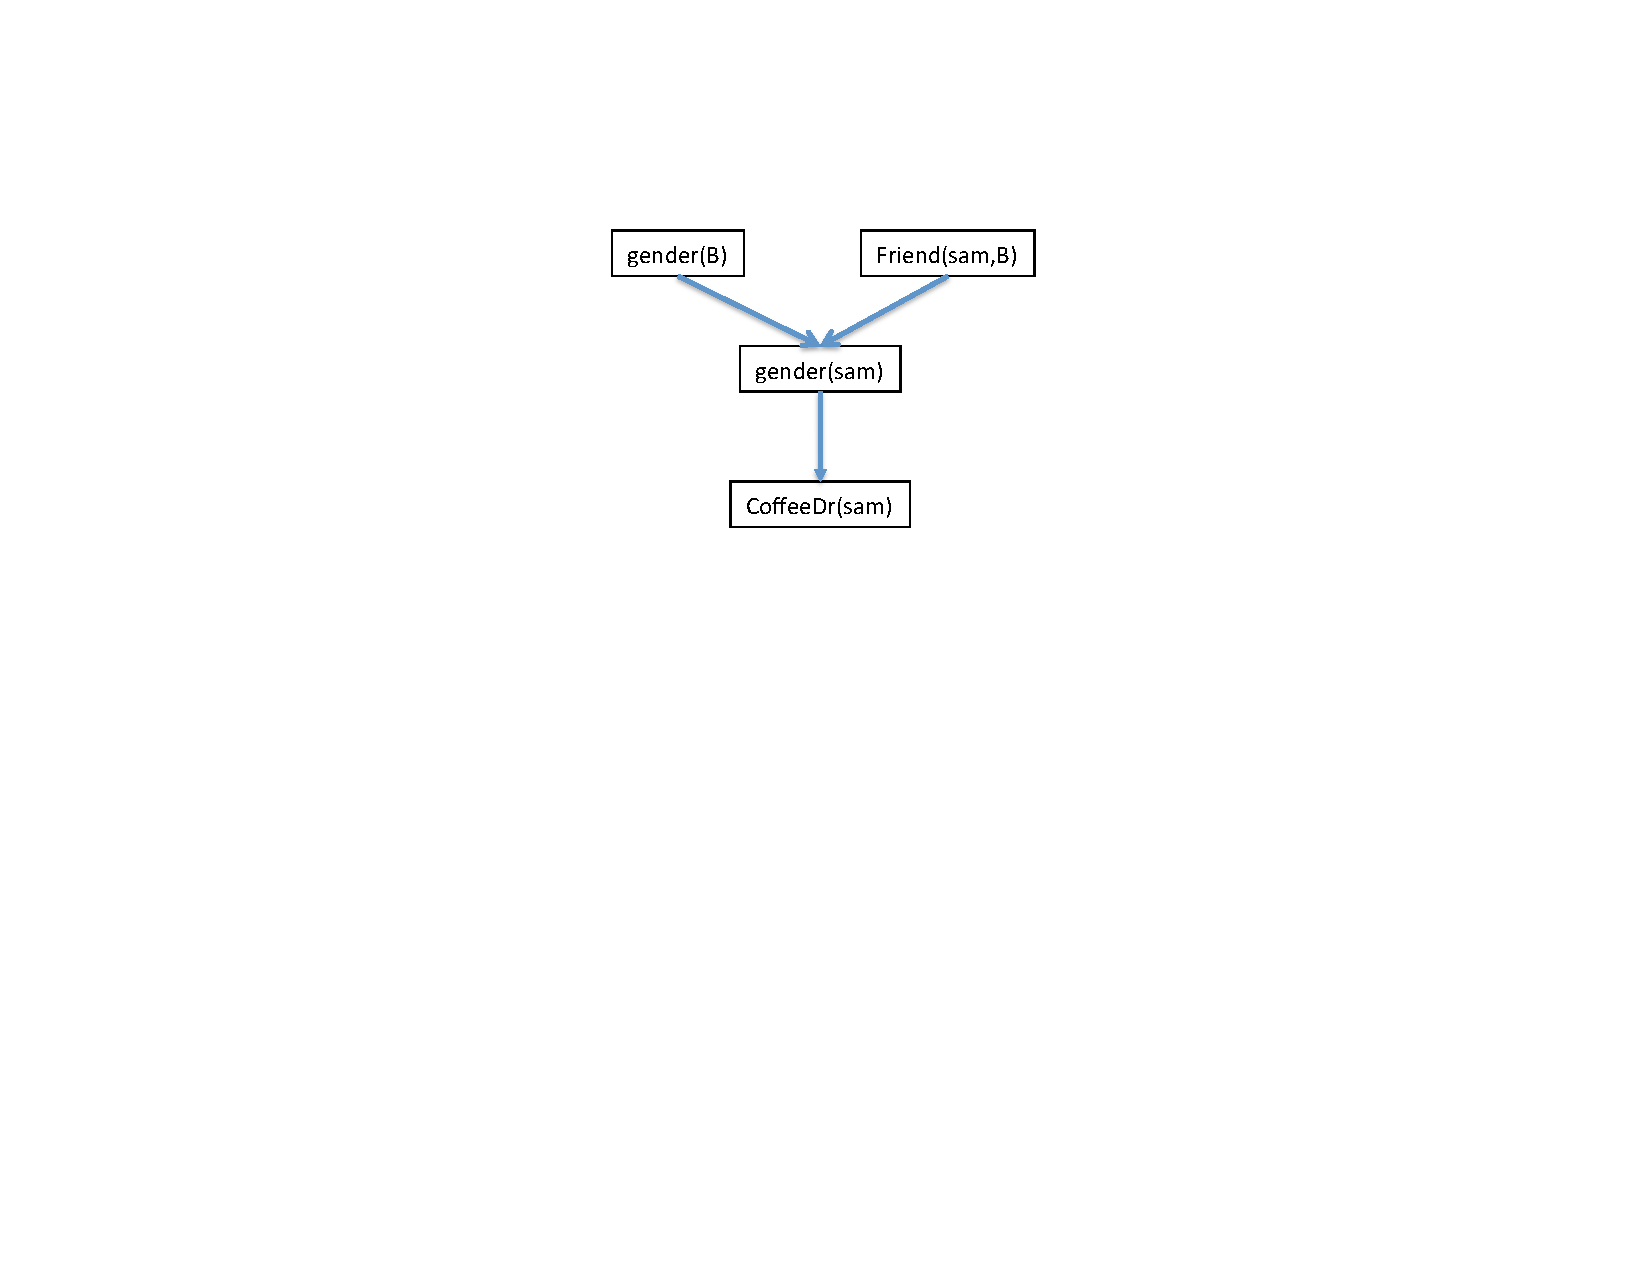
\includegraphics{figures/regression-graph}
%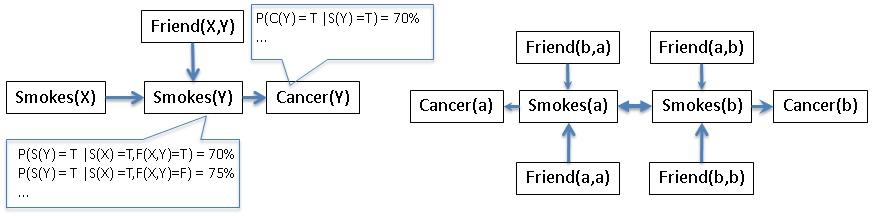
\includegraphics[width=2 \textwidth]{combine1.jpg}
}
\caption{Graphical representation of partial grounding for the target node $\it{gender}(sam)$. The graph results from instantiating the population variable $\A$ with the constant $sam$ in the template graph of Figure~\ref{fig:pbn}. Feature counts are computed with respect to the instantiated nodes. Notice that, for some nodes, this instantiation leads to only a {\em partial} grounding.
\label{fig:regress}}
\end{center}
\end{figure}

Normalizing feature counts to obtain feature frequencies must be done with care to take account of irrelevant features. Since irrelevant features receive log-difference weight 0, they are effectively pruned from the model, so their portion of the instantiation counts should be shifted to the relevant features, analogous to conditioning on relevant features. We therefore define the following two feature functions, where a feature is a family configuration.





\begin{description}
\item[Relevant Count]  The relevant count $\Relevant{\Cvar}$ is 0 if the family configuration is irrelevant; otherwise it is the instantiation count.
\item[Relevant Frequency] The relevant frequency of a feature is its relevant count, divided by the sum of all relevant counts for the same family.
\end{description}

%
%We define the relevant count $\Relevant{\Cvar}$ to be 0 if the query family configuration is irrelevant; otherwise it is the count. 

Algorithm~\ref{alg:relcount} describes the computation of relevant counts and relevant frequencies. Table~\ref{table:log-diff-example} gives examples. 
This completes our definition of the set of features, weights, and feature functions. All told, the resulting log-linear equation is as follows.





\begin{definition}[The Log-Difference Frequency Equation]\label{def:log-diff-freq-eq}
\begin{eqnarray*}
  \Gprob{\FG{\Ground{\TI}} = \TV} {\QC} &\propto &  \\
 \sum_{\UT} \sum_{\UV,\Prange{\UT}}   
\qquad \left[ \ln \cprob{\UT = \UV}{\Pa{\UT} = \Prange{\UT}} \right] &
    \cdot &
    \Relfreq{\Appendterm{\Ground{\UI}  = \UV} {\Ground{\Pa{\UI}} = \Prange{\UT}}} {\Qconj})
%\label{eq:log-diff-freq}
\end{eqnarray*}
where 
\begin{eqnarray*}
\UT &\mbox{varies over} &  \Setaddterm{\TT} {\Ch{\TT}}, \\
\UV & \mbox{varies over} & \Range{\UT}, \quad\mbox{and}\\
\Prange{\UT} & \mbox{varies over} &  \Range{\Pa{\UT}}.
\end{eqnarray*}
\end{definition}


\begin{table}

%\resizebox{1.1\textwidth}{!}{
\begin{tabular}{lrlrrrr|rr}
%%%%%% DO NOT MODIFY THIS FILE DIRECTLY %%%%%%
%%%%%% IT IS GENERATED BY apply-eqs.py %%%%%%
\\\hline
{\setlength{\tabcolsep}{0pt}\begin{tabular}{l}Child \\Value \end{tabular}}&{\setlength{\tabcolsep}{0pt}\begin{tabular}{l} Prior \\ Prob. \end{tabular}}&Parent State&{\setlength{\tabcolsep}{0pt}\begin{tabular}{l} Cond. \\ Prob.\end{tabular}}&$w\;\;$&$\Relevant{\Fvar}$&$w \times \Relevant{\Fvar}$&$\Relevant{\Cvar}$&$w \times \Relevant{\Cvar}$ \\\hline
$cd(sam) = \true$&$0.70\;$&{\setlength{\tabcolsep}{0pt}\begin{tabular}{l}$ g(sam) = \Woman$\end{tabular}}&$0.80\;\,$&$0.13$&$1.0$&$0.13\;\;$&$1$&$0.13\;\;$ \\
$cd(sam) = \false$&$0.30\;$&{\setlength{\tabcolsep}{0pt}\begin{tabular}{l}$g(sam) = \Woman$ \end{tabular}}&$0.20\;\,$&$-0.40$&$0.0$&$0.00\;\;$&$0$&$0.00\;\;$ \\
$g(sam) = \Woman$&$0.45\;$&{\setlength{\tabcolsep}{0pt}\begin{tabular}{l}$ g(B) = \Woman,$\\ $F(sam,B) = \true$\end{tabular}}&$0.55\;\,$&$0.20$&$0.4$&$0.08\;\;$&$40$&$8.02\;\;$ \\
$g(sam) = \Woman$&$0.45\;$&{\setlength{\tabcolsep}{0pt}\begin{tabular}{l}$ g(B) = \Man,$\\ $ F(sam,B) = \true$\end{tabular}}&$0.37\;\,$&$-0.19$&$0.6$&$-0.11\;\;$&$60$&$-11.74\;\;$ \\
$g(sam) = \Woman$&$0.45\;$&{\setlength{\tabcolsep}{0pt}\begin{tabular}{l} n/a\end{tabular}}&$\mathrm{n/a}\;\,$&$-0.79$&$1.0$&$-0.79\;\;$&$1$&$-0.79\;\;$ \\\hline
\multicolumn{6}{l}{Sum ($\ln \Gprob{\it{gender}(sam) = \Woman} {\QC}$)}&$-0.70\;\;$&&$-4.38\;\;$ \\\hline
$cd(sam) = \true$&$0.70\;$&{\setlength{\tabcolsep}{0pt}\begin{tabular}{l}$ g(sam) = \Man$\end{tabular}}&$0.60\;\,$&$-0.15$&$1.0$&$-0.15\;\;$&$1$&$-0.15\;\;$ \\
$cd(sam) = \false$&$0.30\;$&{\setlength{\tabcolsep}{0pt}\begin{tabular}{l}$ g(sam) = \Man$\end{tabular}}&$0.40\;\,$&$0.28$&$0.0$&$0.00\;\;$&$0$&$0.00\;\;$ \\
$g(sam) = \Man$&$0.55\;$&{\setlength{\tabcolsep}{0pt}\begin{tabular}{l}$ g(B) = \Woman,$\\ $F(sam,B) = \true$\end{tabular}}&$0.45\;\,$&$-0.20$&$0.4$&$-0.08\;\;$&$40$&$-8.02\;\;$ \\
$g(sam) = \Man$&$0.55\;$&{\setlength{\tabcolsep}{0pt}\begin{tabular}{l}$ g(B) = \Man,$\\ $ F(sam,B) = \true$\end{tabular}}&$0.63\;\,$&$0.13$&$0.6$&$0.08\;\;$&$60$&$8.14\;\;$ \\
$g(sam) = \Man$&$0.55\;$&{\setlength{\tabcolsep}{0pt}\begin{tabular}{l} n/a \end{tabular}}&$\mathrm{n/a}\;\,$&$-0.59$&$1.0$&$-0.59\;\;$&$1$&$-0.59\;\;$ \\\hline
\multicolumn{6}{l}{Sum ($\ln \Gprob{\it{gender}(sam) = \Man} {\QC}$)}&$-0.75\;\;$&&$-0.63\;\;$ \\\hline

\end{tabular}
%}
\caption{Applying the log-difference frequency equation with the BN of Figure~\ref{fig:pbn} to compute $\Gprob{\it{gender}(sam) = \Woman} {\QC}$ and $\Gprob{\it{gender}(sam) = \Man} {\QC}$. Each row represents a feature/family configuration. For the sake of the example we suppose that the conjunction $\QC$ specifies that Sam is a coffee drinker, has 60 male friends, and 40 female friends.
The last two columns show the result of replacing frequencies by counts (the log-difference count equation in Section~\ref{sec:alternatives}).}
\label{table:log-diff-example}
\end{table}

Whereas in the case of \iid{} data, counts and proportions differ only by a constant population size factor, in relational data there is no such simple one-to-one relationship. For instance Sam and Morgan may each have 10 male friends, but if Sam has 10 friends in total and Morgan has 100 friends in total, the proportion of male friends for Sam is 100\%, whereas for Morgan it is only 10\%. In relational data, normalization involves {\em local} scaling factors (10 for Sam, 100 for Morgan), whereas in i.i.d. data it involves a single glocal factor (the sample size). It is intuitively clear that the count of male friends should be treated very differently in inferences for Sam than in inferences for Morgan. The general problem with using feature counts is that in a log-linear model with counts, features with more instantiations carry exponentially more weight. Count models tacitly conflate number of instantiations with degree of information.
In contrast proportion feature functions are on the common scale [0,1]. Table~\ref{table:log-diff-example} show with count feature functions, factors related to Sam's friend carry much more weight than his/her coffee drinking attribute. 
%
We refer to the diverging scale of feature counts as the \defterm{imbalance problem}. 

\subsection{Estimating Bayes net parameers}

The Bayes net parameters can be estimated using the empirical conditional frequencies observed in an input dataset $\FG{\D}$: The parameter estimate for a family configuration is the number of instantiations of that family configuration in $\FG{\D}$, divided by the sum of all instantiation counts for that family that agree on the parent values and vary the child values. In our notation, the estimate is defined by

\newcommand{\CTPa}{\Count{\Appendterm{\TT = \TV} {\Pa{\TT} = \Prange{\TT}}}  {\FG{\D}}}
\newcommand{\CTPb}{\Count{\Appendterm{\TT = \TV'} {\Pa{\TT} = \Prange{\TT}}}  {\FG{\D}}}

\begin{equation} \label{eq:frequencies}
\estcprob{\TT = \TV} {\Pa{\TT} = \Prange{\TT}} {\FG{\D}} = 
    \frac{\CTPa}
           {\sum_{\TV' \in \Range{\TT}}\CTPb}.
\end{equation}

A theoretical justification for using the observed conditional frequencies is that these estimates maximize a pseudo-likelihood function that measures how well a template BN matches an input dataset \cite{Schulte2011,Schulte2013}. The pseudo-likelihood can be interpreted as the expected value of the log-likelihood of a random grounding of the BN nodes in the template model.

\section{Empirical Comparison of Count vs. Proportion Feature Functions}\label{sec:empirical-comparison}

Our first set of experiments compares the predictive accuracy of the Bayes net log-linear equation \eqref{def:log-diff-freq-eq}, used with counts as feature vs. proportions. The next section describes experiments comparing the Bayes net log-linear equation with functional gradient methods for learning relational dependency networks.

\subsection{Experimental Conditions and Metrics}\label{sec:conditions}

All experiments were done on with 8GB of RAM and a single Intel Core 2 QUAD Processor Q6700 with a clock speed of 2.66GHz (there is no hyper-threading on this chip). The operating system was Linux Centos 2.6.32. Code was written in Java, JRE 1.7.0. All code and datasets are available~\cite{bib:jbnsite}. 

\subsubsection{Datasets}

We describe the datasets in terms of their representation as databases with tables. The databases follow an Entity-Relationship (E-R) design \cite{Ullman1982}. An E-R schema can be translated into our function-based logical notation as follows: Entity sets correspond to populations, descriptive attributes to functions, relationship tables to predicates, and foreign key constraints to type constraints on the arguments of relationship predicates.
%
We used %one synthetic and 
5 benchmark real-world databases from prior work~\cite{Schulte2012}. 
%The databases are fairly complex, so the experiments are computationally demanding, especially the Alchemy inference component, which needs to be applied to all groundings of all descriptive attributes to compute average predictive performance. The databases and their main characteristics are as follows. 
% and on-line sources such as \cite{bib:jbnsite}.
%In this paper we report the average result over all subdatabases in this paper and leave the evaluation of how models should evolve based on the size of data to an extension of the work in a journal paper. 


%{\em University Database.} We manually created a small dataset, based on the schema given in Table~\ref{table:university-schema}.
%The dataset is small and is used as a toy example for testing purposes. There are three entity tables, Student, Course, Professor, and 2 relationship tables RA and Registered.
%The entity tables contain 38 students, 10 courses, and 6  Professors. The $\reg$ table has 92 rows and the $\it{RA}$ table has 25 rows. %This dataset is translated into 513 ground atoms.

\begin{description}

\item[MovieLens Database] This is a standard dataset from the UC Irvine machine learning repository. 
% \cite{Schulte2012}.
%The schema for the dataset is shown in Table \ref{}.
It contains two tables representing entity sets: User with 941 tuples and Item (Movies) with 1,682 tuples.
The User table has 2 descriptive attributes, $\age$ and $\it{gender}$. We discretized the attribute $\age$ into three equal-frequency bins. The table Item represents information about the movies. It has 17 Boolean attributes that indicate the genres of a given movie. There is one relationship table Rated corresponding to a Boolean predicate. The Rated contains Rating as descriptive attribute; 80,000 ratings are recorded.  We performed a preliminary data analysis and omitted genres that have only weak correlations with the rating or user attributes, leaving a total of three genres (Drama, Horror, Action).
%
%The full dataset contains 170,143 ground atoms and is too big for Alchemy to perform learning. We made small subsamples to make the experiments feasible. Subsampling 100 Users and 100 Items transforms to an Alchemy input file with 3,485 ground atoms. Structure learning with Alchemy takes around 30 min.
%Subsampling 300 Users and 300 Items transforms to an Alchemy input file with 27,134 ground atoms. Structure learning with Alchemy takes about 2 days to run.
%The full table with 100,000 ratings exceeded the memory limits of Tetrad, so we randomly picked 40\% of the ratings of the relationship table as input data.

\item[Mutagenesis Database] This dataset is widely used in Inductive Logic Programming research \cite{Srinivasan1996}. %It contains 4 tables total to 15218 tuples. 
We used a previous discretization \cite{Schulte2012}.
Mutagenesis has two entity tables, Atom with 3 descriptive attributes, and Mole (decribing molecules), with 5 descriptive attributes. 
%including two attributes that are discretized into ten values each (logp and lumo).
There are two relationship tables, MoleAtom, indicating which atoms are parts of which molecules, and Bond, which relates two atoms and has 1 descriptive attribute. 
%The full dataset, with 35,973 ground atoms, crashed Alchemy with both structure  and parameter learning. A subsample with 5,017 ground atoms did not terminate for structure learning, but weight learning was feasible. The computational difficulties of Alchemy compared to the MovieLens dataset are  due to the high number of descriptive attributes.
%%another subsample with
%Representing a relationship between entities from the same table in a parametrized Bayes net requires using two or more variables associated with the same population (e.g., $\it{Bond}(\A_{1},\A_{2}))$.
%(Techreport 2009) describes a straightforward extension of Algorithm~\ref{alg:structure} for this case, which we applied to the Mutagenesis dataset.\footnote{Reference omitted for blind review.}
%We also tested our method on the Financial dataset with similar results, but omit a discussion due to space constraints.

\item[Hepatitis Database] This data is a modified version of the PKDD02 Discovery Challenge database \cite{Frank2007}. %, which includes removing tests with null values. 
The database contains information on laboratory examinations of 771 hepatitis B- and C-infected patients, taken
between 1982 and 2001. The data are organized in 7 tables (4 entity tables,  3 relationship tables) with 16 descriptive attributes. They contain basic information about the patients, results of biopsy, information on interferon therapy, results of out-hospital examinations, and results of in-hospital examinations. 

\item[Mondial Database] 
%
%\textbf{Hassan: which version did you use? The full one from http://www.dbis.informatik.uni-goettingen.de/Mondial/mondial-ER.pdf or Bahareh's?} 
%
This dataset contains data from multiple geographical web data sources. 
%Our dataset contains 4 entity tables, $\it{Country},\it{Continent},\it{Economy},\it{Government}$, where the latter three are related to Country by many-one relationships, and one relationship table $\it{Borders}$ that relates two countries.
%This dataset contains data from multiple geographical Web data sources \cite{mondial}. 
We follow the modification of She~\etal~\cite{wangMondial}, and use a subset of the tables and disretized features: 2 entity tables, $\it{Country},\it{Economy}$. The descriptive attributes of Country are continent, government, percentage, majority religion, population size. The descriptive attributes of Economy are inflation, gdp, service, agriculture, industry. A relationship table Economy\_Country specifies which country has what type of economy. A self-relationship table Borders relates two countries.
  %$\it{Country},\it{Continent},\it{Economy},\it{Government}$, where the latter three are related to Country by many-one relationships, and one relationship table $\it{Borders}$ that relates two countries. Our dataset includes a self-relationship table Borders that relates two countries.



\item[UW-CSE database] This dataset lists facts about the Department of Computer Science and Engineering at the University of Washington, such as entities (e.g., $Person$, $Course$) and the relationships (i.e. $AdvisedBy$, $TaughtBy$).
% \cite{Domingos2007}. 
%The total number of ground atoms is 4,106,841. The database contained a total of 3380 ground atoms. 

\end{description}

\subsubsection{Prediction Metrics}
We evaluate the algorithms using classification
accuracy and conditional log likelihood (CLL). These metrics have been used in previous evaluations of MLN learning~\cite{Domingos2007,Schulte2012}.  For each fact $\FG{\TI} = \TV$ in the test dataset, we evaluate the accuracy of the predicted Gibbs probability $\Gprob{\FG{\TI} = \TV} {\QCtarget}$, where $\QCtarget$ is a complete conjunction for all ground terms other than $\FG{\TI}$. Thus $\QCtarget$ represents the values of the input variables as specified by the test dataset.
For classification accuracy, a model's prediction is scored as correct if the true value of the ground term in the test dataset receives the highest Gibbs probability. 
CLL is the average of the logarithm of the Gibbs probability for each fact in the test dataset. Thus $\exp(CLL)$ is the geometric mean of the Gibbs probabilities.\footnote{The geometric mean of a list of numbers $x_{1},\ldots,x_{n}$ is $(\prod_{i} x_{i})^{1/n}$.}
Both metrics are reported as averages over all functors that represent descriptive attributes. For binary predicates we also use Area Under Curve, computed as in \marginpar{fill in reference}.
The learning methods were evaluated using 5-fold cross-validation. Each database was split into 5 folds by randomly selecting entities from each entity table, and restricting the relationship tuples in each fold to those involving only the selected entities  (i.e., subgraph sampling~\cite{Frank1977,Schulte2012}). The models were trained on 4 of the 5 folds, then tested on the remaining one. All results are averages from 5-fold cross validation, over all descriptive attributes in the database. 


\subsubsection{Learning the Bayes Net Structure and Parameters}

All the methods compared in this experiment require a prior Bayes net structure and parameters.
To obtain the structure, the learn-and-join algorithm~\cite{Schulte2012} was applied to each benchmark database. The parameters were computed from the empirical conditional frequencies in the database (Eq.~\ref{eq:frequencies}) using previously-published algorithms~\cite{Schulte2013}. The resulting structure and parameters were used for all methods in this experiment. 
 


\subsection{Results} 

Table~\ref{table:bn} summarizes the results for the Bayes net log-linear model.
The numbers represent an average over many individual scores, one for each fact
%ground literal 
in the database. 
For instance in the biggest dataset, MovieLens, the average is over a total of 170,000 scores; see Table~\ref{table:learn-times}. 

To aid interpretability, we also report the following transformation of CLL: prob. ratio = $\exp(CLL(proportion) - CLL( count))$. This quantity represents the geometric mean, over all test facts, of the fact likelihood ratio of the $\it{proportion}$ feature function over the $\it{count}$ feature function.
For instance, the value of 1.06 for the dataset UW means that on (geometric) average, the likelihood that the $\it{proportion}$ feature function assigns to the correct value for the target node is 1.06 times that assigned by the the $\it{count}$ feature function.


 
\begin{table}[thbp]
\caption{Conditional log-likelihood (log-probabilities) and classification accuracy (in percent) of Bayesian network log-linear equations. We show averages and standard deviations. The probability ratios can be interpreted as the geometric average ratio of likelihoods assigned by the count resp. proportion feature functions to the true target node value.}

%\resizebox{0.5\textwidth}{!}{

\begin{center}
%\resizebox{0.5\textwidth}{!}{
\begin{tabular}{|l|c|c|c|c|c|}
\hline
Accuracy& UW & Mondial & MovieLens & Mutagenesis & Hepatitis \\\hline
 count & 78 $\pm$ 0.08 & 40 $\pm$ 0.05 & 64 $\pm$ 0.01 & 62 $\pm$ 0.05 & 49 $\pm$ 0.03 \\

proportion & \textbf{81} $\pm$ 0.06 & \textbf{45} $\pm$ 0.04 & \textbf{65} $\pm$ 0.01 & \textbf{67} $\pm$ 0.03 & \textbf{55} $\pm$ 0.02 \\
\hline
\end{tabular}
\end{center}

\begin{center}
\begin{tabular}{|l|c|c|c|c|c|}
\hline
CLL & UW & Mondial & MovieLens & Mutagenesis & Hepatitis \\\hline
count & -0.47 $\pm$ 0.10 & -1.47 $\pm$ 0.17 & -1.19 $\pm$ 0.07 & -0.84 $\pm$ 0.03 & -1.33 $\pm$ 0.07 \\
proportion & \textbf{-0.41} $\pm$ 0.04 & \textbf{-1.34} $\pm$ 0.09 & \textbf{-0.71} $\pm$ 0.01 & \textbf{-0.73} $\pm$ 0.04 & \textbf{-1.07} $\pm$ 0.10\\
Prob. ratio & 1.06 & 1.14 & 1.62 & 1.12 & 1.30\\
\hline
\end{tabular}
%}
\end{center}
\label{table:bn}
\end{table}%

Using proportions rather than counts improves the conditional log-likelihood score, substantially on MovieLens and Hepatitis (probability ratio 1.62 resp. 1.30).
Proportions also achieve top performance for  classification accuracy. However, the classification score difference between proportions and counts is small ($<1\%$), except for a bigger improvement (3\%) on MovieLens. Whereas classification accuracy is a 0-1 loss function, CLL is continuous, so balancing factors with proportions has substantially more impact on CLL. In sum:\keypoint{Using Bayes net parameters, proportion feature functions outperform count feature functions.} This finding supports our hypothesis that using proportions as feature functions is an effective way of addressing the imbalance problem.



\section{Comparison with RDN-Boost}
\label{sec:general-weights}

RDN-Boost is a state-of-the-art learner for undirected relational models \cite{Natarajan2012}. We compare the predictive accuracy of RDNs derived from Bayesian networks with those learned by RDN-Boost as a benchmark. RDN-Boost follows the approach of learning a separate discriminative model for each  parametrized random variable in the network. The basic discriminative model is a relational regression tree. RDN-Boost employs functional gradient boosting to learn an ensemble of regression trees for each parametrized random variable. Since RDN-Boost is known to perform well on datasets with relatively few predicates and datapoints, we focus our evaluation on the more complex larger datasets of the previous section. We used the Boostr implementation of RDN-Boost provided by its creators \cite{Khot2013}. The current implementation supports gradient boosting only for binary predicates so our evaluation examines those only. We report results for Boostr's default settings. We experimented with changing some of these settings but changes did not lead to higher accuracy or faster runtimes. We report the performance metrics as computed by Boostr. 




\subsection{Results}

\keypoint{The Bayes net frequency regression predictions are competitive with those from a model with optimized general weights.}

%%UW values are from Zhensong
\point{Accuracy} Table~\ref{table:mbn} shows the scores of the MBN method, together with the log-difference frequency results from Table~\ref{table:bn}. The log-difference frequency model scores slightly higher than the MBN weights on every dataset, with the biggest differences on Mutagenesis (5\%),  MovieLens (5\%) and Hepatitis (4\%). 

\begin{table}[thbp]

\caption{Conditional log-likelihood (log-probabilities) and classification accuracy (percent) of MBN and log-difference frequency predictions.}

\begin{center}

\begin{tabular}{|l|c|c|c|c|c|}
\hline
Accuracy& UW & Mondial & MovieLens & Mutagenesis & Hepatitis \\\hline
MBN & 80 $\pm$ 0.05 & 44 $\pm$ 0.04 & 60 $\pm$ 0.02 & 62 $\pm$ 0.02 & 51 $\pm$ 0.02 \\\hline
log-diff $+$ freq & \textbf{81} $\pm$ 0.06 & \textbf{45} $\pm$ 0.04 & \textbf{65} $\pm$ 0.03 & \textbf{67} $\pm$ 0.03 & \textbf{55} $\pm$ 0.02 \\
\hline
\end{tabular}
\end{center}


\begin{center}
\begin{tabular}{|l|c|c|c|c|c|}
\hline
CLL & UW & Mondial & MovieLens & Mutagenesis & Hepatitis \\\hline
MBN & -0.44 $\pm$ 0.07 & \textbf{-1.28} $\pm$ 0.07 & -0.79 $\pm$ 0.03 & -0.91 $\pm$ 0.09 & -1.18 $\pm$ 0.26 \\
log-diff $+$ freq & \textbf{-0.41} $\pm$ 0.04 & -1.34 $\pm$ 0.09 & \textbf{-0.71} $\pm$ 0.01 & \textbf{-0.73} $\pm$ 0.04 & \textbf{-1.07} $\pm$ 0.10 \\
Prob. ratio & 1.03 & 0.94 & 1.08 & 1.20 & 1.12\\
\hline
\end{tabular}
%}
\end{center}
\label{table:mbn}

\end{table}%


\point{CLL}
The log-difference frequency  model scores better than MBN model on UW, MovieLens, Mutagenesis and Hepatitis (probabilities 3--20\% higher) and scores slightly worse on Mondial (6\% lower probability); see Figure~\ref{fig:summarize}.

\begin{figure}[htbp]

\begin{center}
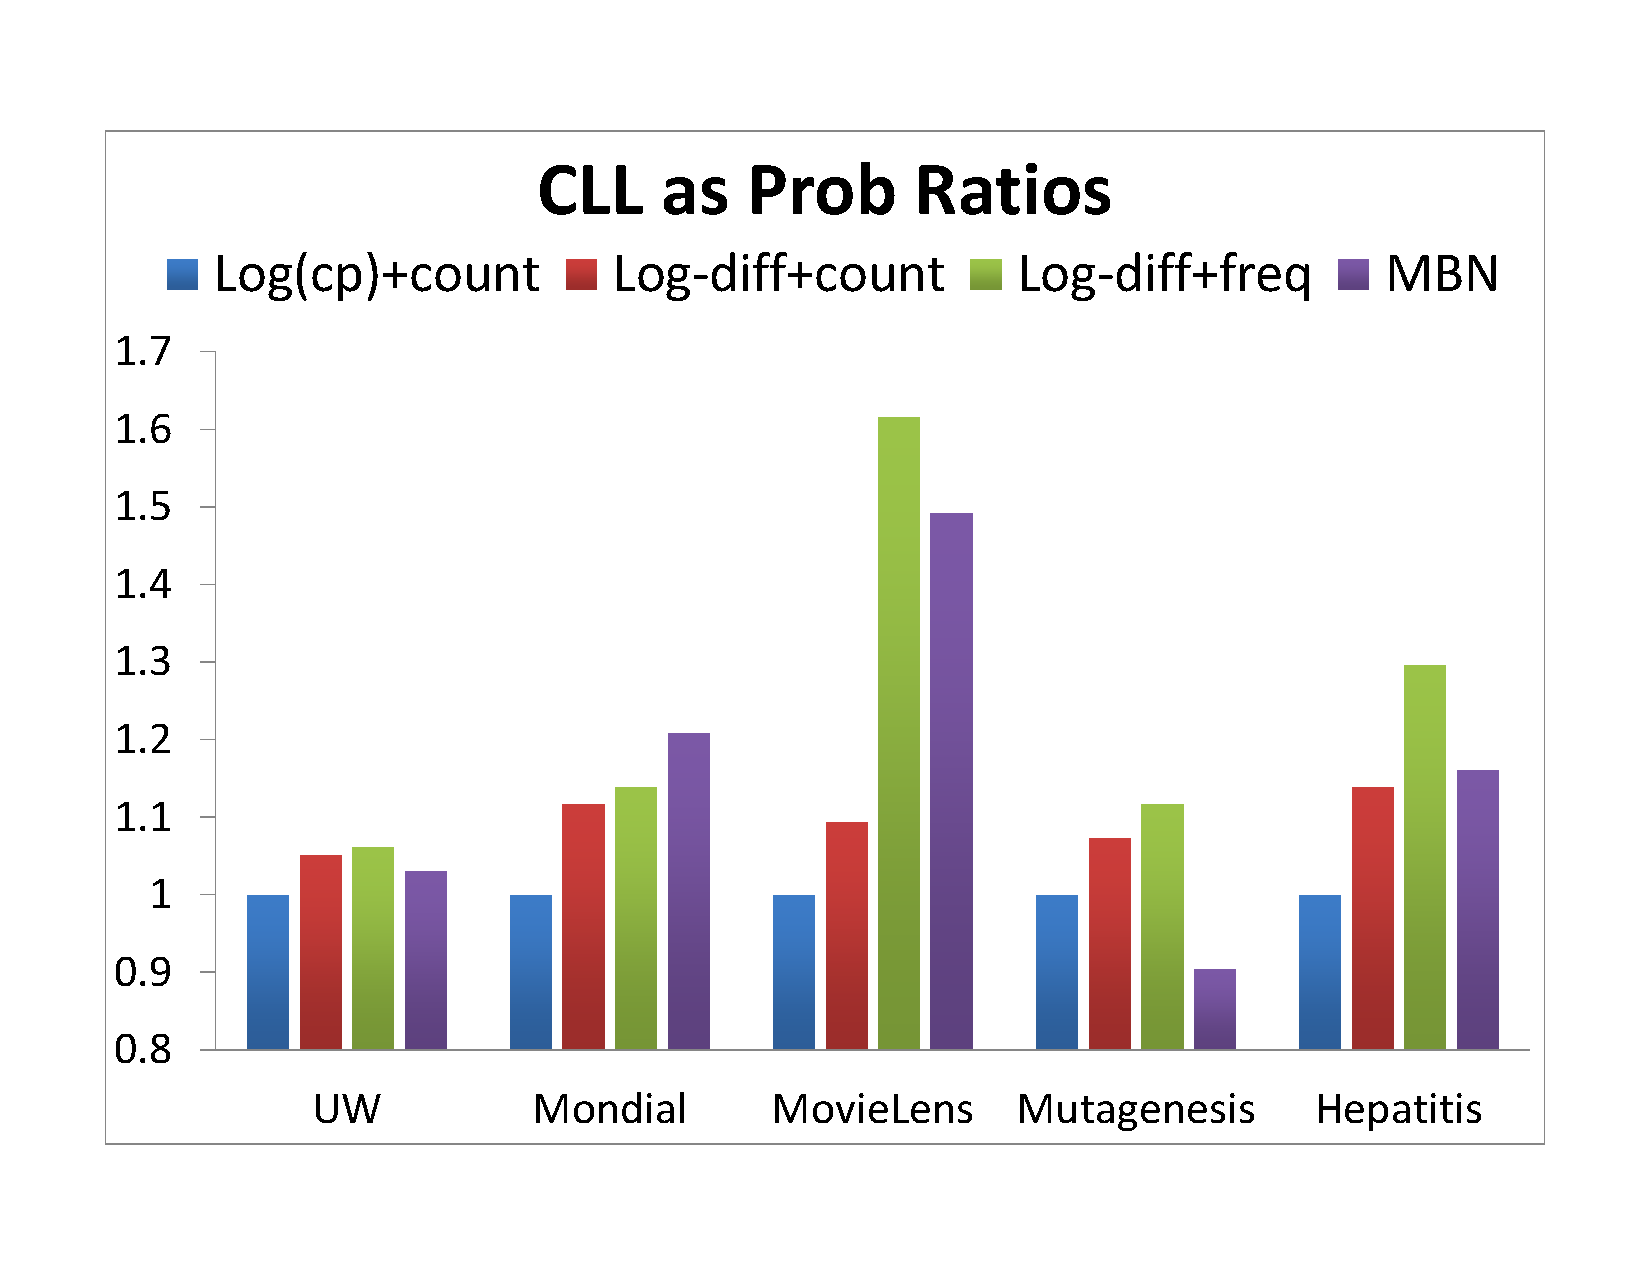
\includegraphics[width=0.6\textwidth]{CLL_Prob_Ratios_New}
%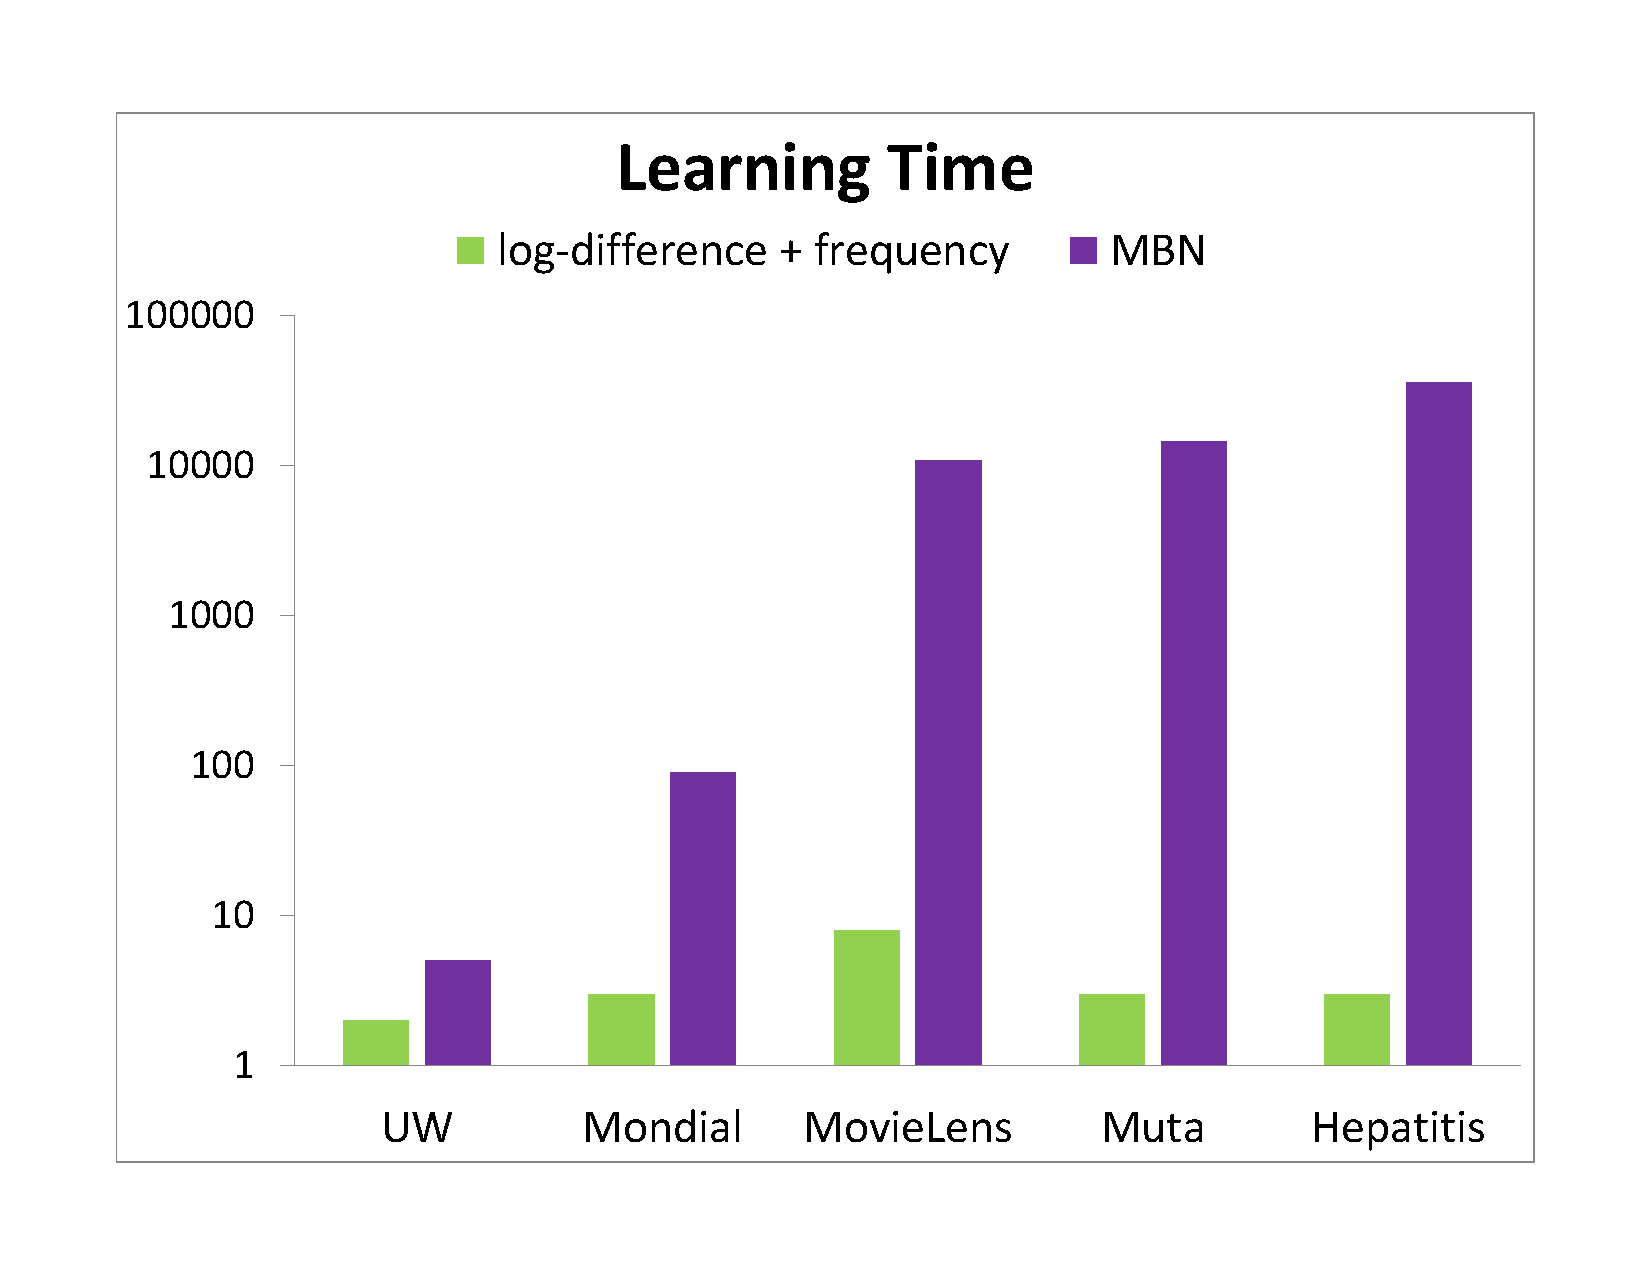
\includegraphics[height=0.5\textheight]{learning_time}
\caption{Predictive Performance averaged over all five benchmark databases. With Bayes net parameters, the frequency model performs better than the count model in terms of likelihood ratios. 
%General weight learning is much slower than Bayes net parameter learning; note that learning times are plotted on a logarithmic scale.
%\fixneeded{Expand ``Prob'' to ``Probability''.}
%\fixneeded{The 2D bars are much better---but they are still darker at the bottom.}
}
\label{fig:summarize}
\end{center}
\end{figure}

\point{Learning Times}
Table~\ref{table:learn-times} shows run time results for structure and parameter learning. We see \keypoint{clear scalability advantages for the maximum likelihood conditional probability estimates used in the Bayes approach}: they take seconds to compute, whereas Alchemy weight optimization requires as much as 10 hours in the worst case (Hepatitis). 

\begin{table}[t]
\caption{Parameter learning times for MBN and Bayes net methods. 
We characterize each database by its counts of ground atoms, tuples,
and Bayes net parameters, and its time for structure learning. The Bayes net
parameter count is the number of family configurations in the Bayes
net.}
\begin{center}
\begin{tabular}{|l r r c c|r c|}
\hline
Dataset & Literals~ & Tuples~  & Parms. & Struct. & MBN~ & Bayes \\
& ($\times 1000$) & ($\times 1000$) & ($\times 10$) & (s) & {(s)\quad} & (s) \\\hline
UW & {3\quad} & {1\quad} & 12 & 36 & 5~~ & \bf{2} \\
Mondial & {2\quad} & {1\quad}  & 58 & 12 & 90~~ & \bf{3}\\
MovieLens & {170\quad} & {82\quad} & 33 & 72 & 10800~~ & \bf{8}\\
Mutagenesis & {35\quad} & {15\quad} & 88 & 30 & 14400~~ & \bf{3}\\
Hepatitis & {71\quad} & {15\quad} & 79 & 24 & 36000~~ & \bf{3}\\\hline
\end{tabular}
\end{center}
\label{table:learn-times}
\end{table}


\point{Discussion} The prediction scores provide evidence that dependency networks learned via Bayesian networks achieve accuracy that is competitive with state-of-the-art dependency network learners. Another advantage of Bayesian networks is that the predictions can be easily interpreted in terms of a log-linear model and local conditional probabilities. Classifier ensembles are more difficult to interpret; the RDN-Boost creators note that ``we sacrifice comprehensibility for better predictive performance''. There are a number of possibilities for combining the advantages of Bayesian network learning with gradient boosting: [copy from introduction]


 
 





 

\section{Conclusion and Future Work} 
\label{sec:conclusion}

This paper presented a new log-linear inference equation for applying Bayes nets to relational data. For a fixed template Bayes net, the equation defines the Gibbs conditional probability of a target node given an assignment of values to all other nodes. A log-linear model is defined by: a set of features, and for each feature, a feature function and a feature weight. The predicted conditional probability is the exponentiated weighted sum of feature function values. In our proposed model, the features are all family configurations in for a family in the Bayes net, whose child node is either the target node or a child of the target node. The weight associated with a child-parent feature is computed as the log-difference of two quantities determined by the BN parameters: (i) the conditional probability of the child value, given its parent configuration, and (ii) the marginal probability of the child value. The feature function is the frequency with which the feature is instantiated in the given query, normalized with respect to relevant features only. 

Our experiments on five benchmark datasets compared our log-difference frequency equation to several alternatives: using counts as feature frequencies, and  using log-conditional probabilities as feature weights. We also compared using transformed Bayes net parameters as weights to using weights directly learned from the data by log-linear optimization methods. Our frequency equation achieved the best predictive performance on all but one dataset. Using the maximum likelihood values as Bayes net parameters is much faster than optimizing weights using standard log-linear methods (Markov Logic), typically seconds vs. hours. 
%The impact of using Bayes net structures was compared to structure learning with the state-of-the-art MLN-Boost method. Bayes net learning was much faster than the boosting approach, with competitive predictive accuracy.

Different model classes each have their advantages and disadvantages. Nonetheless  the combination of Bayes nets and  our proposed log-linear model,  offers a unique set of advantages compared to other inference methods for multi-relational data, in terms of the  \emph{interpretability} and \emph{scalability} of both structure and parameter learning: Feature weights are readily interpreted as a log-transformation of the Bayes net conditional probability parameters, and the Bayes net parameters can be computed in closed-form as the empirical frequencies. 

We have established novel connections between the use of frequency feature functions and what, at first sight, appear to be unrelated issues such as the imbalance problem, pruning irrelevant features, maximum likelihood estimation, and the random selection interpretation of template Bayes nets. (1) The imbalance problem arises because feature instantiation counts in relational data can diverge by orders of magnitude. Rescaling counts as frequencies produces feature function values on the same scale. According to our experiments, changing the feature function is a more effective approach to the imbalance problem than using the weight parameters to rescale (assign smaller weight magnitudes to larger feature counts). (2) It is important not only to prune irrelevant features, but also to define instantiation frequencies over the space of relevant features only. (3) Maximum likelihood estimation is competive with optimizing weight parameters from the data only when relevant feature frequencies are used as feature functions. (4) Under mild assumptions, our frequency equation is equivalent to a {\em random selection} method, where the prediction score for a target node value is defined as the expected score, with respect to a random instantiation of the template Bayes net, computed using the standard Bayes net equation for a Gibbs conditional probability.

There are several avenues for future work. While we focus on Bayes nets, the imbalance problem arises also for other relational models. Our solution of changing the predictor space from counts to frequencies applies to log-linear models in general.
\cite{Sutton2007,Taskar2002,Domingos2009}.
The frequency equation can be combined with other log-linear learning methods, for example within a model ensemble. Functional gradient boosting \cite{Khot2011} is a powerful technique for learning such ensembles. 

Our model introduces a 1-1 correspondence between log-linear weights and Bayes net parameters. Therefore log-linear regularization techniques \cite{Huynh2008} can be used for smoothing parameter estimates in template Bayes nets, and for detecting irrelevant features. 

Local Gibbs probability models  may be inconsistent in the sense that there is no joint distribution that agrees with the local conditional probabilities \cite{Heckerman2000}. An open theoretical question is whether our local frequency equations for different target nodes are guaranteed to be mutually consistent. If they are inconsistent, a possible approach is to apply the recent averaging methods for dependency networks \cite{Lowd2012,Poole2013}.

Our log-linear equation with relevant feature frequencies appears to be a principled, fast-to-learn, and accurate model for relational prediction with Bayes nets.




\section*{Acknowledgements} This work was supported by Discovery Grants to Oliver Schulte from the Natural Science and Engineering Council of Canada. Zhensong Qian was supported by a grant from the China Scholarship Council. A preliminary versions of this paper was presented at the StarAI 2012 workshop. We are indebted to workshop reviewers and participants for helpful comments.
\bibliographystyle{plain}
\bibliography{master}
\end{document}
